\documentclass[a4paper,11pt,twocolumn]{article}

% — Core Typography & Formatting —
\usepackage[utf8]{inputenc}
\usepackage[T1]{fontenc}
\usepackage[english]{babel}
\usepackage{microtype}
\usepackage{geometry}
\usepackage{parskip}
\usepackage{titlesec}
\usepackage{xcolor}
\usepackage{lineno}

% — Mathematics —
\usepackage{amsmath}
\usepackage{amssymb}
\usepackage{dsfont}

% — Tables, Figures & Graphics —
\usepackage{graphicx}
\usepackage{subcaption}
\usepackage{booktabs}
\usepackage{tabularx}
\usepackage{float}
\usepackage{caption}
\usepackage{siunitx}
\usepackage{tikz}
\usetikzlibrary{positioning, fit, arrows.meta, shapes.geometric, backgrounds, calc}

% — Color & Hyperlinks Settings —
\definecolor{darkblue}{rgb}{0.0, 0.0, 0.55}
\usepackage[colorlinks=true, allcolors=darkblue, urlcolor=darkblue]{hyperref}

% — Citations & Referencing —
\usepackage{csquotes}
\usepackage[numbers, square, sort&compress]{natbib}
\usepackage{authblk}
\usepackage{orcidlink}

% — Layout Configuration —
\geometry{
	top=20mm,
	bottom=20mm,
	left=15mm,
	right=15mm,
	columnsep=6mm
}

\sisetup{
	group-separator = {.},
	output-decimal-marker = {,},
	detect-all
}

\captionsetup{font=small, labelfont={bf,color=darkblue}}

% — Section Formatting —
\titleformat{\section}{\normalfont\large\bfseries\color{darkblue}}{\thesection}{1em}{}
\titleformat{\subsection}{\normalfont\normalsize\bfseries}{\thesubsection}{1em}{}
\titleformat{\paragraph}[runin]{\normalfont\normalsize\bfseries}{}{0em}{}[.]
\titlespacing*{\section}{0pt}{1.5ex plus 1ex minus .2ex}{1ex plus .2ex}
\titlespacing*{\subsection}{0pt}{1.2ex plus 1ex minus .2ex}{0.8ex plus .2ex}

% ==============================================================================
% TITLE & AUTHOR BLOCK
% ==============================================================================
\title{Decoding Secondary Lymphomas: Integrating Macro-Epidemiological Models and Micro-Genomic Signatures to Disentangle Mutagenesis from Misdiagnosis}
\date{\today}

\begin{document}
	
	\makeatletter
	\twocolumn[
	\begin{@twocolumnfalse}
		\begin{center}
			\vspace*{-0.5cm}
			{\Large \textbf{Disentangling Mutagenesis from Misdiagnosis in Secondary Lymphomas: An Integrated Macro-Epidemiological and Transcriptomic Framework}}
			
			\vspace{0.8cm}
			
			{\small 
				\textbf{Pietro Grassi}\textsuperscript{1} \orcidlink{0009-0006-5569-4398},
				\textbf{Elena Bariletti}\textsuperscript{2} \orcidlink{0009-0001-4812-6652}
			}
			
			\vspace{0.3cm}
			
			{\footnotesize 
				\textit{\textsuperscript{1}Honours Student of Data Science at Sant'Anna School of Advanced Studies, Pisa, Italy} \\
				\textit{\textsuperscript{2}Honours Student of Biotechnology at Sant'Anna School of Advanced Studies, Pisa, Italy} \\
			}
			
			\vspace{0.8cm}
			
			\begin{minipage}{0.88\textwidth}
				\small \textbf{Summary}
				
				\vspace{0.2cm}
				
				Secondary Non-Hodgkin Lymphoma (sNHL) following Hodgkin Lymphoma (HL) carries a dismal prognosis and was canonically attributed to delayed treatment-induced mutagenesis. While contemporary hematopathology increasingly recognizes the role of shared clonal evolution and diagnostic blind spots, the magnitude of initial molecular misdiagnosis remains under-quantified. We deployed a dual-scale computational framework to disentangle true mutagenesis from baseline molecular misdiagnosis. Macro-epidemiologically, Cause-Specific Cox and Fine-Gray competing-risk architectures applied to the SEER registry ($N=\num{45530}$) revealed that baseline clinical severity—rather than systemic chemotherapy ($p=0.339$)—is the dominant etiological driver of sNHL incidence. Micro-genomically, utilizing a nested stability-selection penalized regression pipeline on independent T-cell lymphoma cohorts (GSE19069), we distilled a highly robust 22-gene signature. Anchored by the T-follicular helper cytokine IL-21, this signature effectively distinguished Angioimmunoblastic T-cell Lymphoma (AITL) from other peripheral phenotypes (external validation on GSE58445 reaching $\operatorname{AUC} = 0.890$). Crucially, topological projection of an independent classical HL cohort (GSE17920) demonstrated profound transcriptomic overlap with the AITL continuum. These findings empirically validate ``morphological mimicry'': the heavy reactive background of occult AITL indistinguishably mimics HL under standard morphological evaluation. Consequently, apparent rapid-onset therapy-related lymphomas are often pre-existing misclassified clones, mandating a transition toward proactive molecular interception in initial diagnostic protocols.
				
				\vspace{0.5cm}
				\noindent \textbf{Keywords:} Secondary Non-Hodgkin Lymphoma; Competing Risks; Transcriptomics; Misdiagnosis.
				\vspace{0.5cm}
				
				\noindent \textbf{Statements and Declarations:} The authors declare no conflict of interest.
				\vspace{0.5cm}
				
				\noindent \textbf{Funding:} The authors received no external funding.
			\end{minipage}
		\end{center}
		\vspace{0.8cm}
		\hrule
		\vspace{0.8cm}
	\end{@twocolumnfalse}
	]
	\makeatother
	
	% ==============================================================================
	% MAIN MANUSCRIPT
	% ==============================================================================
	
	\section{Introduction}
	
	The therapeutic evolution of primary Hodgkin Lymphoma (HL) stands as a benchmark of success in modern hematology, with long-term survival rates now surpassing 80\% \cite{Ansell2015, Schaapveld2015}. However, this dramatic extension of the life-cycle has exposed a critical clinical vulnerability: the emergence of secondary Non-Hodgkin Lymphomas (sNHL). These subsequent malignancies impose a devastating mortality burden—with 5-year survival rates often below 40\%—presenting a phenotype characterized by extreme chemoresistance and aggressive clinical trajectories \cite{Eichenauer2021}.
	
	Historically, the pathogenesis of secondary malignancies post-HL was broadly conceptualized under the umbrella of iatrogenic mutagenesis \cite{Morton2013}. While this genotoxic paradigm holds robust predictive power for secondary myeloid neoplasms like acute myeloid leukemia \cite{Morton2013}, large population studies suggest that the etiology of secondary lymphomas is more complex, strongly implicating therapy-induced immunosuppression rather than isolated DNA damage \cite{Schaapveld2015}. Consequently, epidemiological registries such as SEER frequently categorize these events as ``therapy-related neoplasms'' based solely on their temporal sequence. However, recent advances in molecular pathology suggest that this macroscopic categorization is etiologically oversimplified \cite{Alaggio2022}. Emerging evidence indicates that a substantial fraction of rapid-onset sNHLs—such as Peripheral T-cell Lymphomas (PTCL) and Angioimmunoblastic T-cell Lymphoma (AITL)—may not represent true treatment-induced events, but rather the clinical unmasking of occult clones that were misclassified at baseline \cite{Swerdlow2016, Alaggio2022}.
	
	AITL, in particular, represents a diagnostic ``blind spot'' due to its profound morphological and microenvironmental mimicry of HL. Both entities share a polymorphous inflammatory background and the presence of Epstein-Barr virus (EBV)-positive B-cell blasts that can indistinguishably resemble Hodgkin and Reed-Sternberg cells \cite{Swerdlow2016}. Standard diagnostic protocols, relying on static morphology and limited immunohistochemistry, are often ill-equipped to capture the underlying T-follicular helper (Tfh) transcriptomic machinery that distinguishes aggressive AITL from primary HL \cite{deLeval2007, Swerdlow2016}. This lack of molecular granularity leads to suboptimal initial stratification and the eventual, seemingly abrupt emergence of a supposedly secondary, refractory T-cell lymphoma.
	
	Disentangling iatrogenic immunosuppression and mutagenesis from molecular misdiagnosis requires a dual-scale analytical architecture capable of bridging population-level trends with high-resolution transcriptomic data. Methodological silos have historically prevented this synthesis: large-scale registries lack genomic depth, while specialized omics cohorts lack the longitudinal power to model competing mortality risks \cite{Penberthy2024}. 
	
	In this study, we propose an integrated computational framework to resolve this ambiguity. At the macro-epidemiological level, we employ a dual-model survival architecture (Fine-Gray and Cause-Specific Cox models) on the SEER registry ($N=45,530$) to demonstrate that baseline clinical heterogeneity outweighs therapeutic exposure as a driver of sNHL incidence. Concurrently, at the micro-genomic level, we utilize a stability-selected, ultra-high-dimensional penalized regression pipeline to isolate a robust 22-gene transcriptomic signature that distinguishes AITL from other PTCL phenotypes. By projecting primary HL cohorts onto this signature, we empirically quantify the degree of morphological mimicry. Our results suggest that a significant proportion of early-onset secondary lymphomas represent the clinical unmasking of pre-existing aggressive sub-clones, demanding a paradigm shift from reactive epidemiological observation to proactive molecular interception.
	
	\section{Theoretical Framework}
	
	Historically, the pathogenesis of therapy-related neoplasms following HL was presumed to rely exclusively on the direct mutagenic effects of antineoplastic regimens, as alkylating agents and radiotherapy induce direct DNA double-strand breaks. However, landmark population studies have challenged this dogma for lymphoid malignancies; rather than a strict dose-dependent association with specific cytotoxic agents, the elevated risk of sNHL strongly implicates profound iatrogenic and disease-intrinsic immunosuppression \cite{Schaapveld2015}. In the context of secondary T-cell malignancies, prolonged exposure to cytotoxic regimens and chronic antigenic stimulation fosters a profoundly dysregulated immune microenvironment. This persistent immune evasion provides a permissive niche for the aberrant expansion of T-follicular helper (Tfh) cells and the subsequent disruption of normal germinal center architecture \cite{Alaggio2022, Lemonnier2012}.
	
	While this macro-environmental collapse elegantly explains delayed, late-onset sNHL, it fundamentally fails to account for rapid-onset, refractory trajectories. For these early events, the frontier of molecular pathology points toward a complex interplay of clonal hematopoiesis and microenvironmental orchestration. Advanced sequencing has revealed that pre-malignant progenitors harboring early somatic mutations (e.g., TET2, DNMT3A) can lay the groundwork for divergent neoplastic clones \cite{Odejide2014}. Crucially, neoplastic Tfh cells in Angioimmunoblastic T-cell Lymphoma (AITL) actively secrete specific cytokines—such as IL-21 and CXCL13—that recruit a massive polymorphous inflammatory infiltrate. This aberrant cytokine milieu frequently drives the expansion of reactive, Epstein-Barr Virus (EBV)-positive B-cell blasts that serve as prominent ``bystander'' cells within the tumor microenvironment \cite{deLeval2007, Swerdlow2016}.
	
	Integrating these microenvironmental dynamics with the inherent spatial limitations of standard pathological evaluation exposes a critical diagnostic vulnerability: Morphological Mimicry. The presence of large, EBV-positive B-blasts—which strikingly resemble classical Hodgkin and Reed-Sternberg (HRS) cells—set against a rich reactive background of eosinophils, plasma cells, and histiocytes, makes AITL morphologically indistinguishable from classical HL on standard H\&E and limited immunohistochemistry panels \cite{Attygalle2002, deLeval2007, Swerdlow2016}. If comprehensive T-cell clonality assays and Tfh-specific markers (e.g., CD4, PD-1, ICOS) are omitted during the initial biopsy, the underlying T-cell neoplasm is easily eclipsed by the visually dominant HRS-like blasts. Consequently, if a presumptively indolent classical HL already harbors an occult aggressive T-cell transcriptomic machinery, its rapid ``emergence'' as a refractory sNHL is not a \textit{de novo} iatrogenic event, but the devastating clinical unmasking of a misdiagnosed primary AITL clone.
	
	\section{Methods}
	
	A comprehensive mathematical formalization of the algorithms employed is provided in Appendix \ref{app:methodology}.
	
	\subsection{SEER Registry Analysis}
	We queried the SEER database to extract a primary cohort of patients diagnosed with HL. Within this cohort, sNHL was defined as a subsequent primary malignancy. To reflect the clinical reality of survivorship, the follow-up time was calculated from the date of initial HL diagnosis to the onset of sNHL, death from any cause (competing event), or last follow-up (right-censoring). Crucially, to prevent the confounding inclusion of synchronous or composite lymphomas, a strict 6-month latency wash-out period was enforced; any sNHL diagnosed within 6 months of the primary HL was excluded from the event count.
	
	Analyzing population-level trajectories in cohorts of HL survivors introduces survival analysis challenges. Patients treated for HL face a substantial risk of non-cancer-related mortality, primarily cardiovascular events \cite{Aleman2003}. In this context, standard Kaplan-Meier estimators and Cox Proportional Hazards models violate the assumption of independent right-censoring. Treating death as a standard censoring event mathematically forces the assumption that a deceased patient could still develop sNHL if they had lived, thereby overestimating the true cumulative incidence of the secondary malignancy \cite{Austin2016}.
	
	To resolve this mathematical artifact, our framework deployed a dual-model competing risk architecture. For predictive incidence modeling, we directly computed the 10-year cumulative incidence function (CIF) using Fine-Gray subdistribution hazard models \cite{Fine1999}. This approach properly maintains individuals who experience competing events (death) within the risk set, weighted by their probability of surviving without the event of interest. Age was modeled continuously via restricted cubic splines (3 degrees of freedom) to capture non-linear hazard trajectories, while therapeutic interventions and advanced stage were treated as categorical predictors. Conversely, to address the purely etiological question of whether therapeutic interventions directly increase the biological hazard of lymphomagenesis, we fitted Cause-Specific Cox models \cite{Andersen2012}, treating competing deaths as independent censoring to isolate the pure mutagenic signal. Model robustness was evaluated post-estimation: proportional hazards assumptions were verified via Schoenfeld residuals, and prognostic accuracy was assessed through a decile-by-decile 10-year calibration analysis.
	
	To address non-random missingness in staging and treatment data without introducing survival bias, we utilized Multiple Imputation by Chained Equations (MICE). The Nelson-Aalen cumulative hazard estimator and event status were embedded directly into the imputation process to ensure that true time-to-event dynamics intrinsically informed the imputation geometry \cite{White2009}. Following imputation, we identified unbiased clinical phenotypes via Factor Analysis of Mixed Data (FAMD) computed specifically on six core baseline covariates: continuous age, sex, race, advanced clinical stage, chemotherapy, and radiotherapy. The number of latent clusters was systematically evaluated via the Silhouette method. To prevent over-stratification and preserve clinical interpretability, the algorithm was constrained to a local mathematical optimum ($K=11$), mapping patients into distinct ``vulnerability zones'' based on their multi-dimensional profiles.
	
	\subsection{Transcriptomic Signature Discovery and Misdiagnosis Projection}
	The transition from macroscopic incidence to transcriptomic validation requires navigating the curse of dimensionality ($n \ll p$), where the number of transcriptomic features vastly exceeds the number of clinical samples. Standard generalized linear models collapse in this regime due to perfect multicollinearity and inflated variance \cite{Hastie2015}.
	
	Working with the primary T-cell lymphoma microarray cohort (GSE19069), we partitioned the data into an 80\% training set and a 20\% internal hold-out set to prevent data leakage. Missing transcriptomic probes were inferred using a $k$-Nearest Neighbors ($k$-NN) algorithm \cite{Troyanskaya2001}. Crucially, this imputation manifold was computed exclusively within the training set, ensuring the hold-out data remained entirely naive to the training distribution.
	
	To isolate an etiology-defining molecular signature without succumbing to algorithmic overfitting, our methodology leveraged a nested stability selection protocol. We initiated dimensionality reduction via Sure Independence Screening (SIS) \cite{Fan2008}, a marginal correlation-based algorithm proven to possess the ``sure screening property''—reducing dimensionality asymptotically close to the true sparse model. To implement stability selection, this screening was embedded across $B=100$ stratified subsampling iterations \cite{Meinshausen2010}. Features were retained for the core signature only if their selection frequency met the rigorous theoretical consensus threshold of $\ge 50\%$.
	
	The final predictive model was trained using an Elastic Net penalized regression framework \cite{Zou2005}, mixing Ridge ($L_2$) and Lasso ($L_1$) penalties at $\alpha = 0.5$ to optimally balance feature sparsity with the retention of correlated biological pathways. The signature's diagnostic threshold was subsequently optimized on the internal hold-out set using the Youden Index derived from its Receiver Operating Characteristic (ROC) curve.
	
	To evaluate cross-cohort translational robustness, the trained signature was applied to an independent external dataset (GSE58445). To bypass systemic memory crashes associated with $k$-NN imputation on degraded external arrays, a robust median-imputation rescue procedure was implemented prior to harmonization. An orthogonal Empirical Bayes strategy (ComBat) was then applied to neutralize systemic batch effects \cite{Johnson2007}. The GSE19069 training cohort was explicitly designated as the immutable reference batch, projecting the GSE58445 samples strictly into the established training space without altering original model parameters.
	
	Finally, to directly test the hypothesis of ``morphological mimicry'', an independent cohort of pure Classical Hodgkin Lymphoma (GSE17920) was harmonized and topologically projected onto the extracted AITL/PTCL-NOS principal component space. This cross-disease projection empirically quantifies the transcriptomic overlap between primary HL and aggressive T-cell phenotypes, assessing the fundamental probability of baseline molecular misdiagnosis.
	
	\section{Results}
	
	\subsection{Macro-Epidemiological Analysis: Clinical Complexity Outweighs Iatrogenic Mutagenesis}
	
	The macro-epidemiological cohort comprised $N=45,530$ patients diagnosed with primary HL extracted from the SEER registry, strictly filtered to enforce a 6-month latency wash-out period to exclude synchronous composite lymphomas. The baseline characteristics are detailed in Table \ref{tab:supp_baseline} (Appendix \ref{app:materials}).
	
	Unsupervised latent phenotyping via FAMD mapped the multidimensional structure of the cohort. The Silhouette algorithm determined a local mathematical optimum of $K=7$ clusters (Figure \ref{fig:clusters}A), manually chosen to balance complexity and accuracy. The topological projection of these phenotypes (Figure \ref{fig:clusters}B) illustrates a dense, overlapping central manifold. By explicitly removing non-random administrative missingness (e.g., unknown racial status) from the algorithmic feature space, the unsupervised projection confirms that primary HL patients do not stratify into rigid, isolated silos. Instead, they exist entirely on a multidimensional ``clinical continuum''. This geometric continuity validates our epidemiological modeling strategy: the transition to a high-risk sNHL candidate is not a discrete step, but is dictated by subtle, continuous variations across age, stage, and therapeutic intensity.
	
	\begin{figure}[htbp]
		\centering
		\begin{minipage}{\columnwidth}
			\centering
			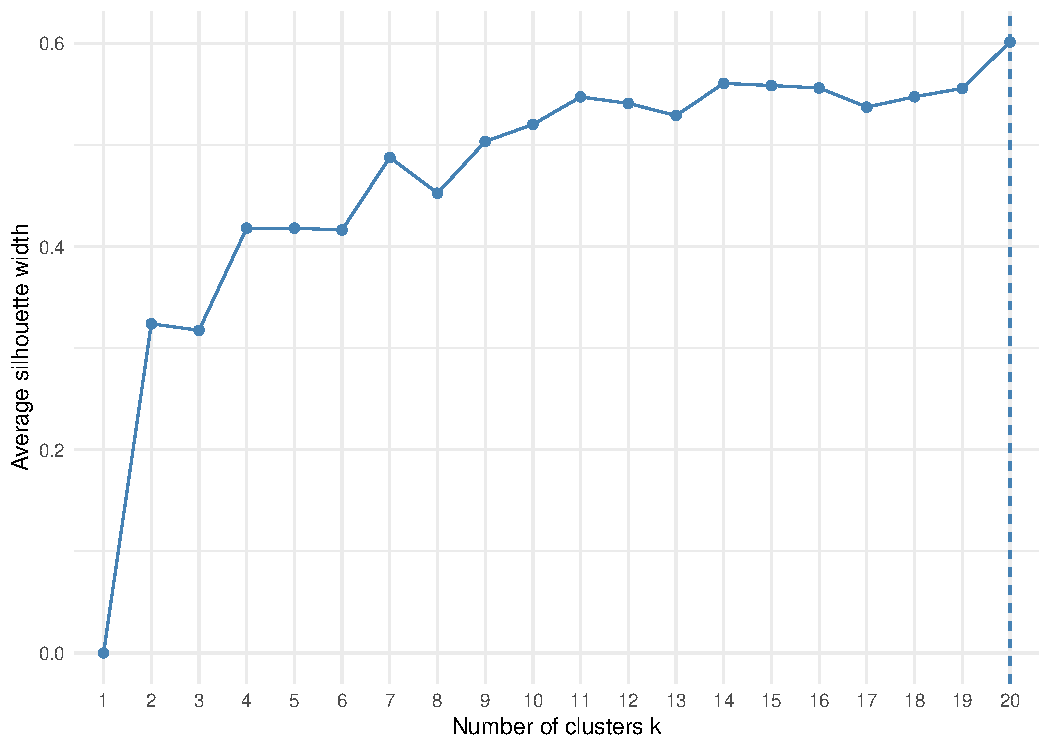
\includegraphics[width=\columnwidth]{Figure3A_Silhouette_Optimal_K.pdf}
			\caption*{A: Optimal K Extraction}
		\end{minipage}\hfill
		\vspace{0.5cm}
		\begin{minipage}{\columnwidth}
			\centering
			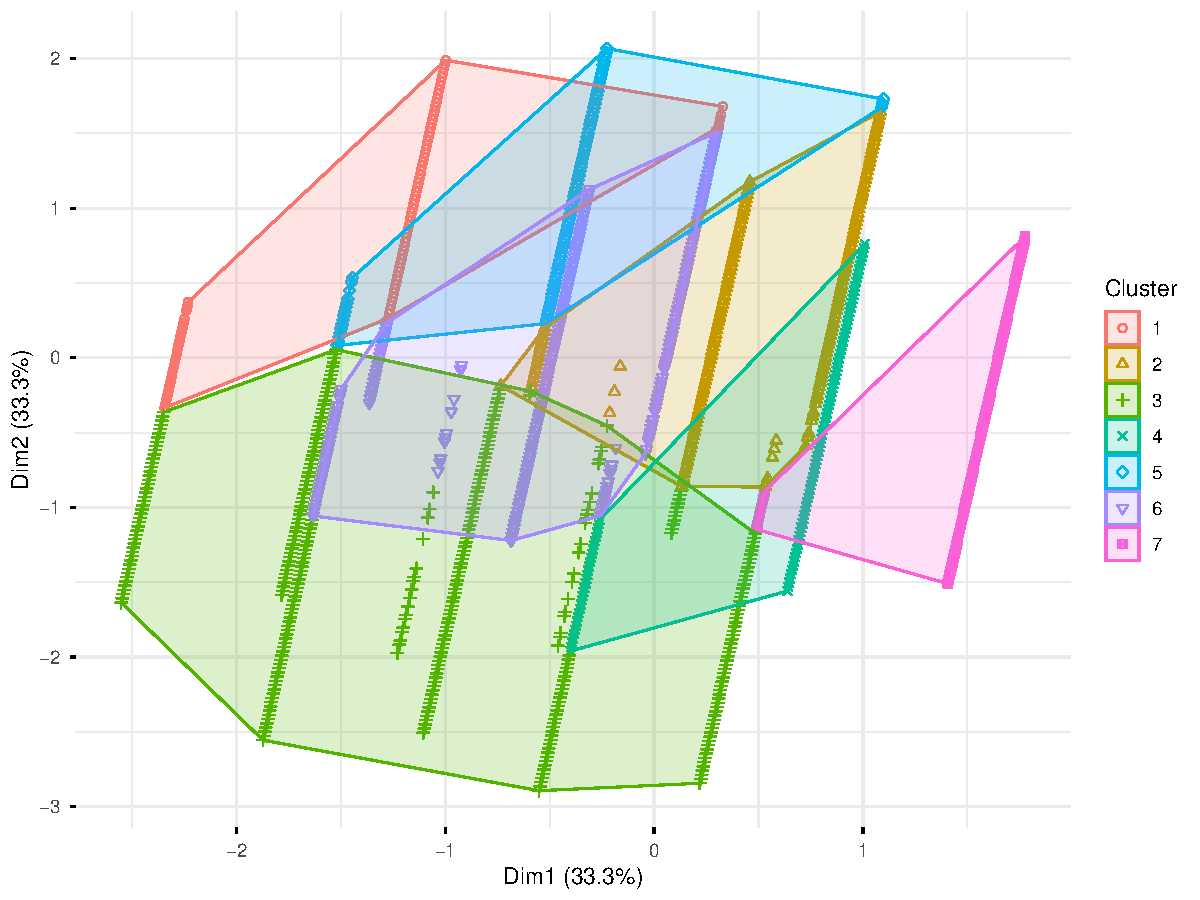
\includegraphics[width=\columnwidth]{Figure3B_Latent_Clusters.pdf}
			\caption*{B: Latent Clinical Phenotypes}
		\end{minipage}
		\caption{Unsupervised clinical phenotyping. (A) Silhouette statistic identifying $K=20$ as the optimum. (B) FAMD topological projection demonstrating the overlapping continuum of latent patient phenotypes.}
		\label{fig:clusters}
	\end{figure}
	
	Evaluating the long-term cumulative incidence of sNHL, while strictly accounting for the competing mortality risk, demonstrated an early overlap of trajectories across therapeutic modalities, which only began to diverge profoundly after a decade of follow-up (Figure \ref{fig:cif}). Patients receiving combined modality therapy (Chemotherapy + Radiotherapy) ultimately maintained the lowest cumulative probability of sNHL.
	
	\begin{figure}[htbp]
		\centering
		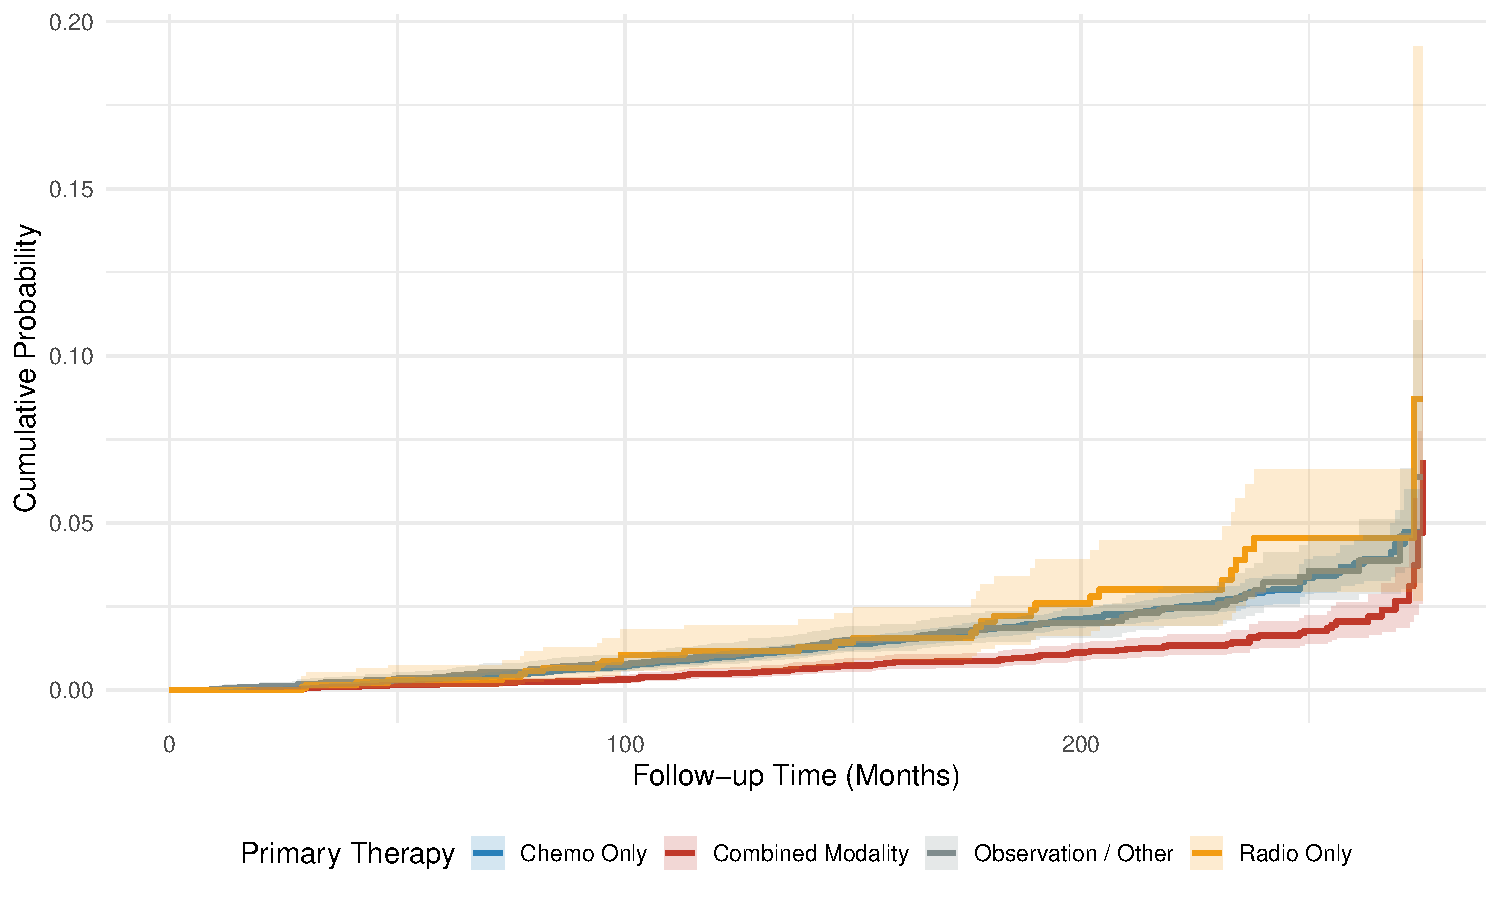
\includegraphics[width=\columnwidth]{Figure1_CIF_Trajectories.pdf}
		\caption{Cumulative Incidence Function (CIF) of secondary NHL, stratified by primary therapeutic modality. Curves are estimated utilizing the Fine-Gray competing risk framework under multiple imputation ($m=5$).}
		\label{fig:cif}
	\end{figure}
	
	The Fine-Gray subdistribution hazard models (Table \ref{tab:finegray}) revealed the paradox of survivorship. When the competing risk of death is incorporated, standard oncological drivers lose their predictive power. The massive mortality rate associated with advancing age and severe clinical presentation drastically abbreviates the patient life-cycle, fundamentally precluding the biological manifestation of late-onset lymphomas. This highlights excellent model calibration at 10 years (Figure \ref{fig:calibration}), indicating a high degree of mathematical agreement between predicted and observed probabilities under missing-data uncertainty.
	
	\begin{table}[htbp]
		\centering
		\caption{Pooled Fine-Gray Subdistribution Hazard Ratios for Secondary NHL.}
		\label{tab:finegray}
		\resizebox{\columnwidth}{!}{
			\begin{tabular}{lccc}
				\toprule
				\textbf{Predictor} & \textbf{sHR} & \textbf{95\% CI} & \textbf{p-value} \\ 
				\midrule
				Chemotherapy (Treated vs Untreated) & 0.18 & 0.02 -- 1.86 & 0.518 \\
				Radiation (Treated vs Untreated) & 0.95 & 0.77 -- 1.18 & 0.783 \\
				Stage (Advanced vs Early) & 1.36 & 1.13 -- 1.64 & 0.356 \\
				Sex (Male vs Female) & 1.14 & 0.96 -- 1.36 & 0.510 \\
				Age (Spline Basis 1) & 9.30 & 2.64 -- 32.75 & 0.342 \\
				Age (Spline Basis 2) & 0.51 & 0.01 -- 36.74 & 0.842 \\
				Age (Spline Basis 3) & 2.03 & 0.76 -- 5.40 & 0.520 \\
				\bottomrule
			\end{tabular}
		}
	\end{table}
	
	\begin{figure}[htbp]
		\centering
		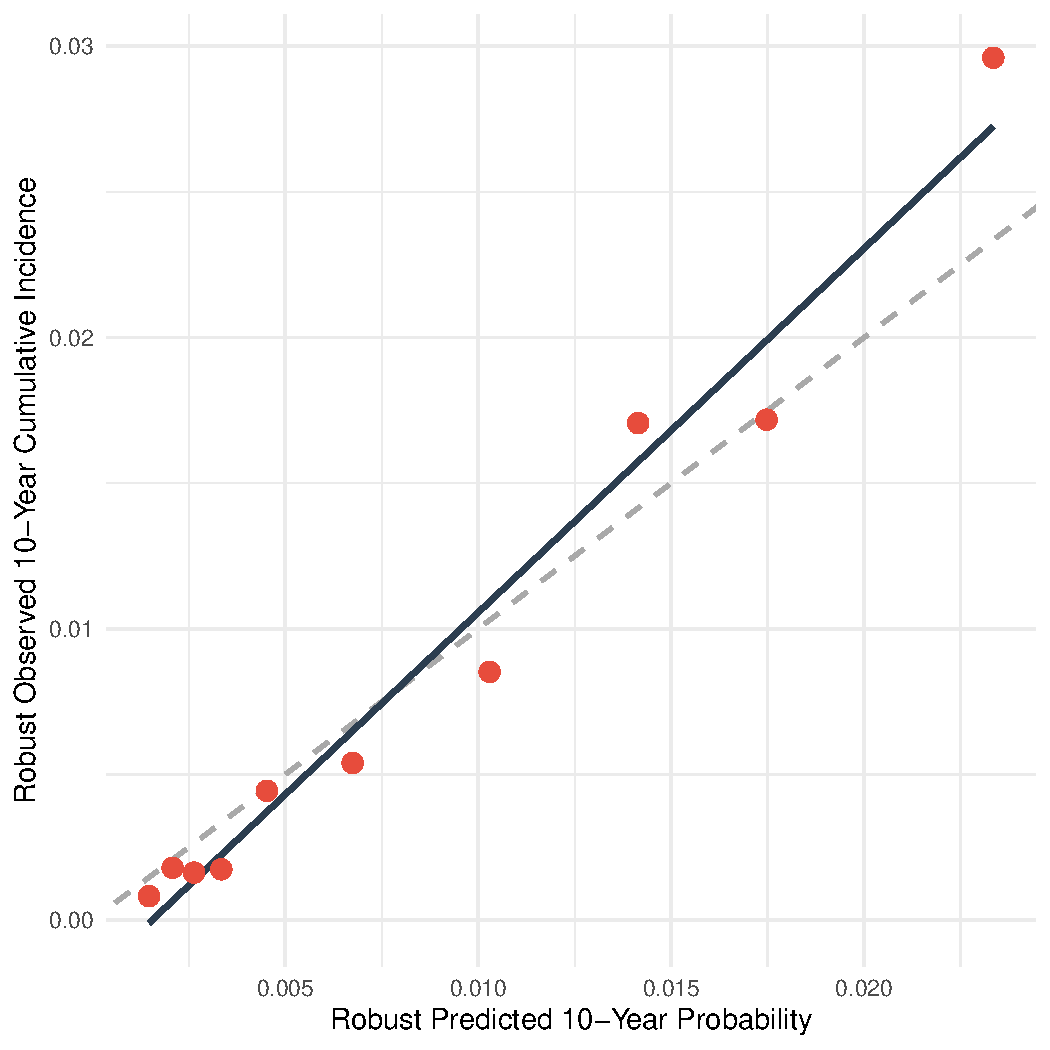
\includegraphics[width=\columnwidth]{Figure5_Calibration_Plot.pdf}
		\caption{10-Year Model Calibration. Predicted mean probabilities versus observed robust cumulative incidence across risk deciles.}
		\label{fig:calibration}
	\end{figure}
	
	To disentangle the pure mutagenic effect from these survival artifacts, the Cause-Specific Cox model (Table \ref{tab:cscox}) isolated the direct biological hazard of sNHL evolution. Crucially, the main effect of systemic chemotherapy did not reach statistical significance ($p=0.339$), forcefully contradicting the historical assumption of its universal mutagenic role in secondary lymphomagenesis. Instead, advanced primary stage ($\operatorname{csHR}=2.06$, $p<0.001$) and non-linear age dynamics emerged as the true etiological drivers (Figure \ref{fig:forest}). This profound influence of baseline clinical severity over systemic iatrogenic exposure strongly reinforces the hypothesis that pre-existing tumor biology (occult aggressiveness) is the actual architect of early-onset secondary lymphomas.
	
	\begin{table}[htbp]
		\centering
		\caption{Pooled Cause-Specific Hazard Ratios (Etiological Drivers).}
		\label{tab:cscox}
		\resizebox{\columnwidth}{!}{
			\begin{tabular}{lccc}
				\toprule
				\textbf{Predictor} & \textbf{csHR} & \textbf{95\% CI} & \textbf{p-value} \\ 
				\midrule
				Chemotherapy (Treated vs Untreated) & 0.25 & 0.01 -- 4.30 & 0.339 \\
				Radiation (Treated vs Untreated) & 0.75 & 0.61 -- 0.93 & 0.007 \\
				Stage (Advanced vs Early) & 2.06 & 1.68 -- 2.51 & $<0.001$ \\
				Sex (Male vs Female) & 1.31 & 1.10 -- 1.56 & 0.002 \\
				Age (Spline Basis 1) & 9.73 & 2.22 -- 42.61 & 0.003 \\
				Age (Spline Basis 2) & 12.24 & 0.06 -- 2701.63 & 0.363 \\
				Age (Spline Basis 3) & 52.42 & 15.50 -- 177.29 & $<0.001$ \\
				\bottomrule
			\end{tabular}
		}
	\end{table}
	
	\begin{figure}[htbp]
		\centering
		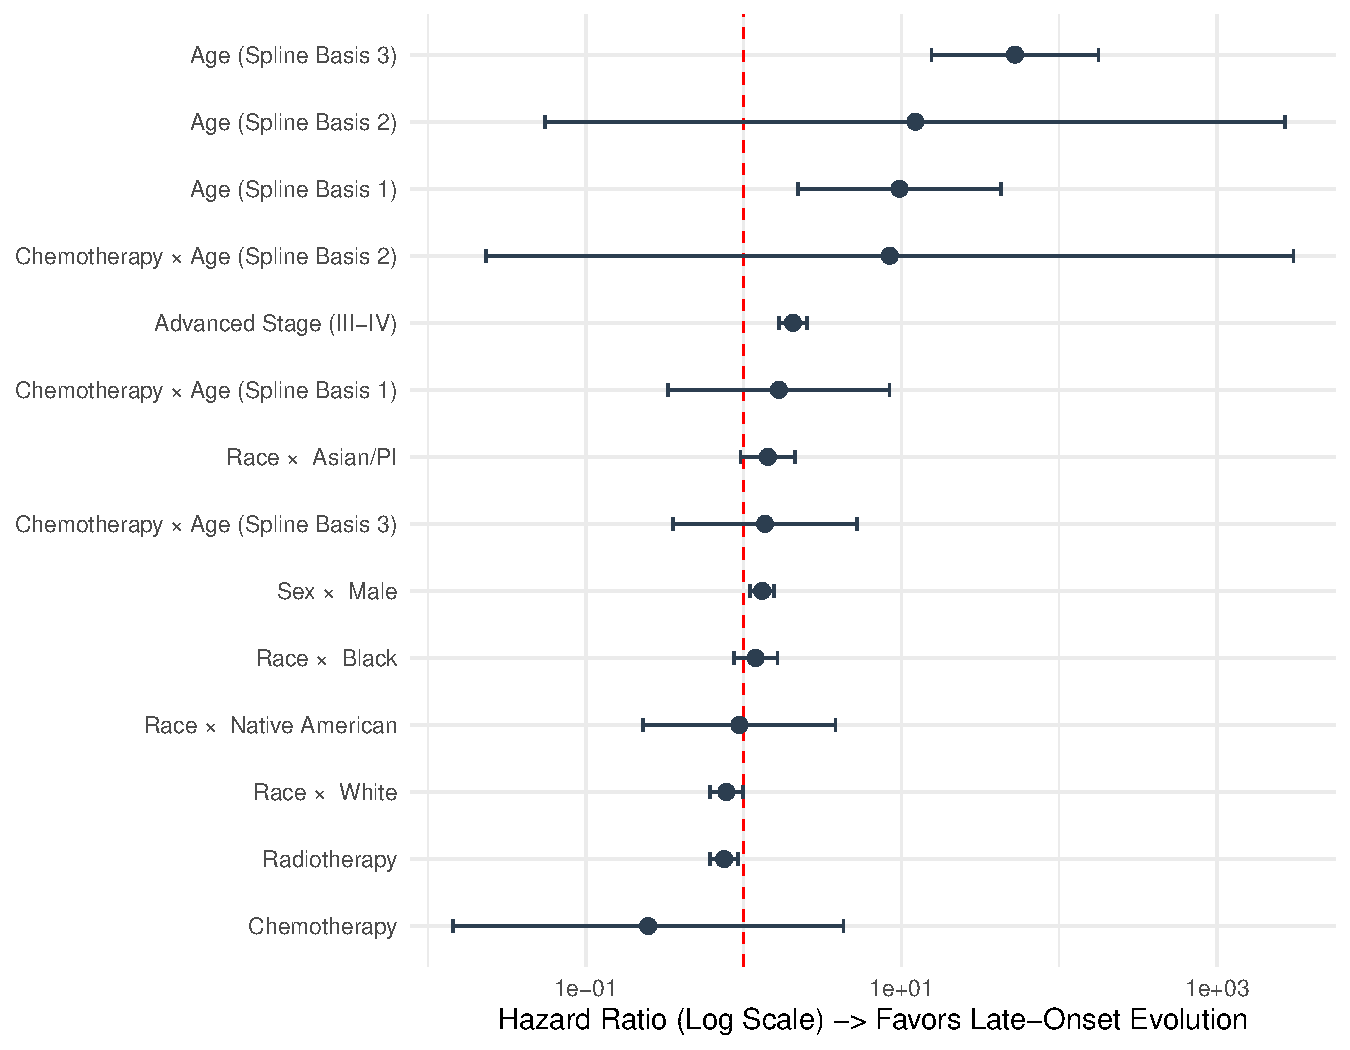
\includegraphics[width=\columnwidth]{Figure2_Etiology_ForestPlot.pdf}
		\caption{Forest Plot of Etiological Drivers. Cause-Specific Cox modeling isolates the direct hazard of mutagenic clonal evolution.}
		\label{fig:forest}
	\end{figure}
	
	\subsection{Micro-Genomic Signatures and the Proof of Morphological Mimicry}
	
	Transitioning to the molecular level to investigate the biology of these ``occult'' aggressive clones, the Nested SIS and stability selection pipeline was executed on the T-cell lymphoma training cohort (GSE19069). Imposing a strict theoretical consensus threshold ($\ge 50\%$ selection frequency across $B=100$ subsampling iterations) successfully distilled the massive transcriptomic space down to a highly robust 22-gene Core Signature. Notably, C9orf47 emerged with ``Ultra Stability'' (91\% frequency), while IL-21—a hallmark cytokine defining T-follicular helper (Tfh) cells—achieved ``High Stability'' (81\% frequency), providing robust biological validation of the signature's capacity to trace the Tfh-cellular origin of AITL.
	
	\begin{figure}[htbp]
		\centering
		\begin{minipage}{\columnwidth}
			\centering
			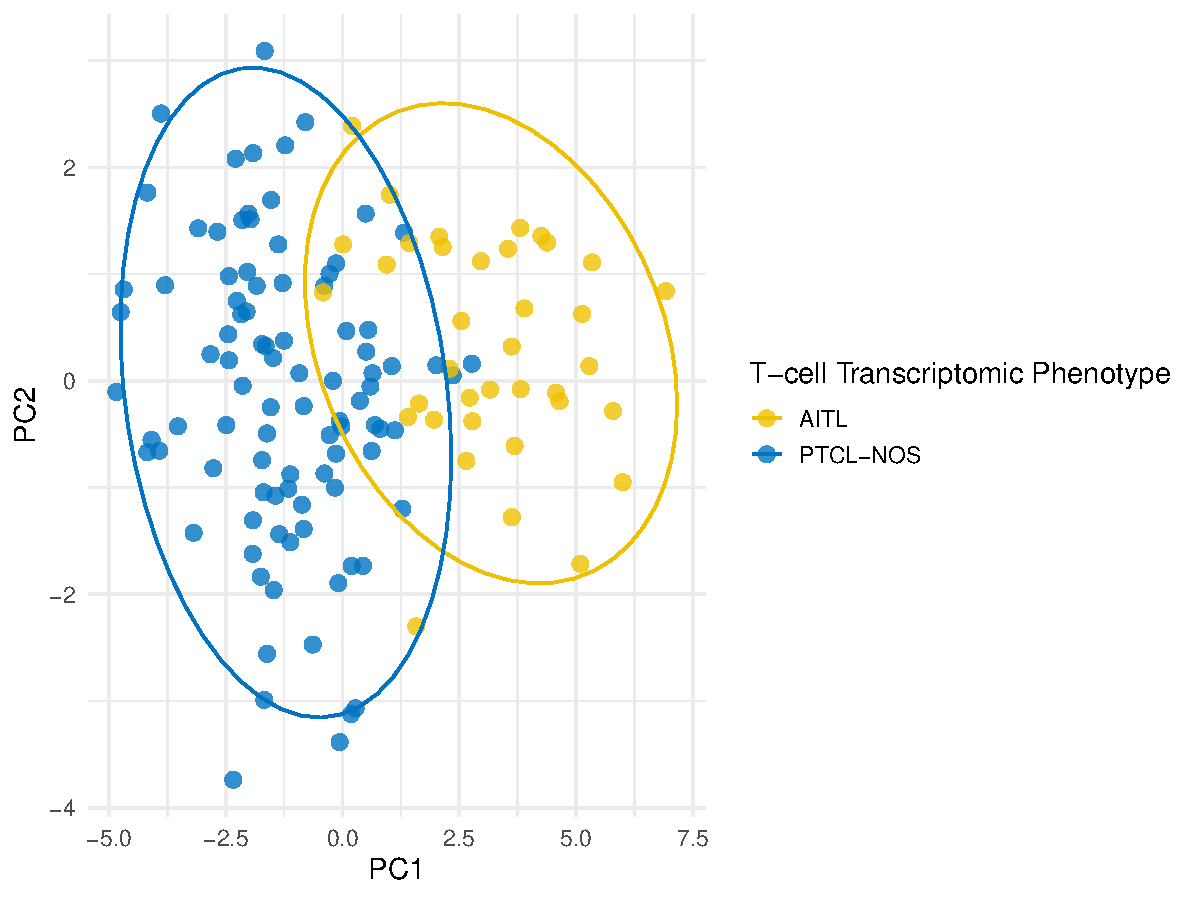
\includegraphics[width=\columnwidth]{Figure1_Unsupervised_PCA.pdf}
			\caption*{A: Unsupervised PCA}
			\vspace{0.5cm}
		\end{minipage}
		\begin{minipage}{\columnwidth}
			\centering
			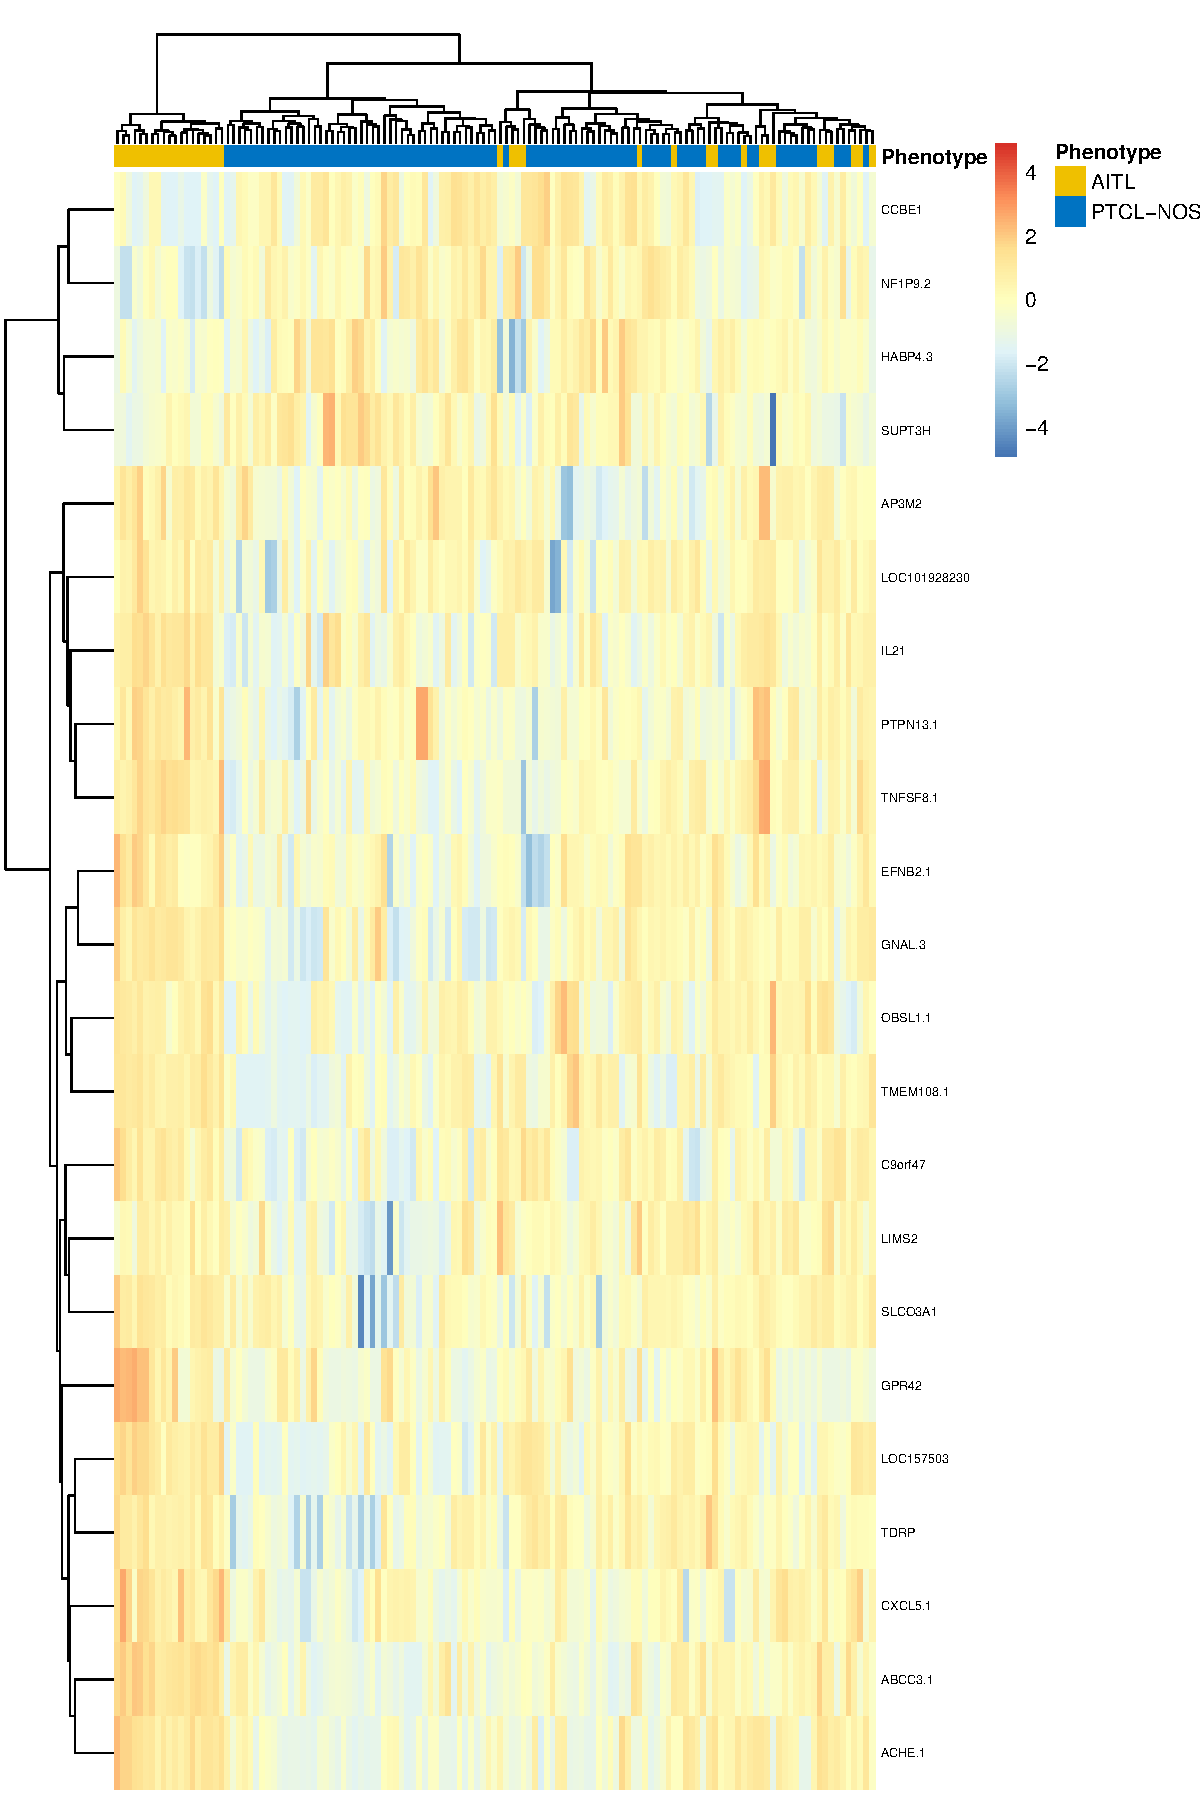
\includegraphics[width=\columnwidth]{Figure2_Genomic_Heatmap.pdf}
			\caption*{B: Hierarchical Clustering}
		\end{minipage}
		\caption{The 22-gene stable transcriptomic signature separating AITL and PTCL-NOS phenotypes.}
		\label{fig:genomic_separation}
	\end{figure}
	
	Unsupervised dimensionality reduction (Figure \ref{fig:genomic_separation}A) and hierarchical clustering (Figure \ref{fig:genomic_separation}B) demonstrated a natural biological stratification of AITL versus PTCL-NOS phenotypes based solely on this 22-gene panel. Gene Set Enrichment Analysis (GSEA) confirmed the underlying systemic shifts (Figure \ref{fig:pathway}), linking the aggressive AITL phenotype to complex cellular machinery dysregulation.
	
	\begin{figure}[htbp]
		\centering
		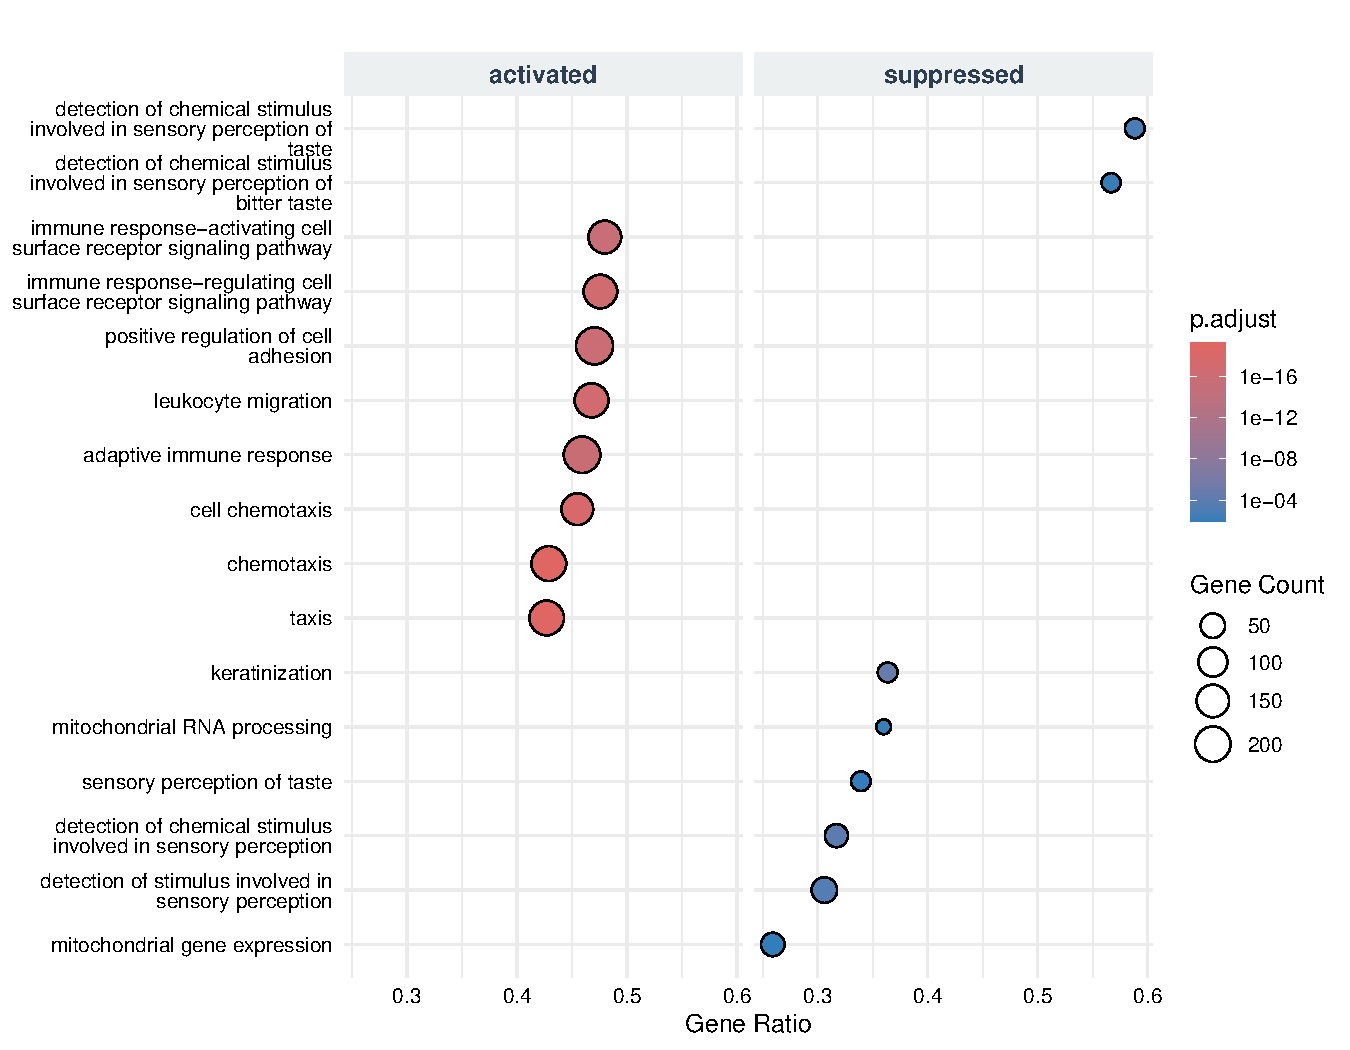
\includegraphics[width=\columnwidth]{Figure4_Pathway_Enrichment.pdf}
		\caption{Gene Set Enrichment Analysis (GSEA). Dotplot highlighting the systemic biological shifts distinguishing the transcriptomic phenotypes.}
		\label{fig:pathway}
	\end{figure}
	
	The diagnostic robustness of this signature was initially assessed on the internal hold-out set (20\% of GSE19069, $n=26$). The model achieved an internal $\operatorname{AUC}$ of 0.875 (Figure \ref{fig:roc_curves}A). While the overall reclassification accuracy was high (Table \ref{tab:reclass}), we acknowledge the inherent statistical limitation of this internal partition, which contained only 4 true AITL cases due to natural class imbalances. A sample size this restricted fundamentally limits the confidence intervals of internal sensitivity and risks overestimating model generalization. 
	
	To overcome this vulnerability and rigorously prove the absolute suppression of high-dimensional overfitting, the trained signature was translated to the independent, large-scale external validation cohort (GSE58445, $N=193$) post-ComBat Empirical Bayes harmonization. Strikingly, the signature's performance not only remained stable but marginally increased to an $\operatorname{AUC}$ of 0.890 (Figure \ref{fig:roc_curves}B). Applying the exact mathematical threshold optimized on the internal cohort, the genomic reclassification of this massive external set (Table \ref{tab:reclass_ext}) provided definitive confirmation that the 22-gene signature captures true, generalizable biological taxonomy, successfully flagging atypical clinical trajectories across distinct populations.
	
	\begin{figure}[htbp]
		\centering
		\begin{minipage}{\columnwidth}
			\centering
			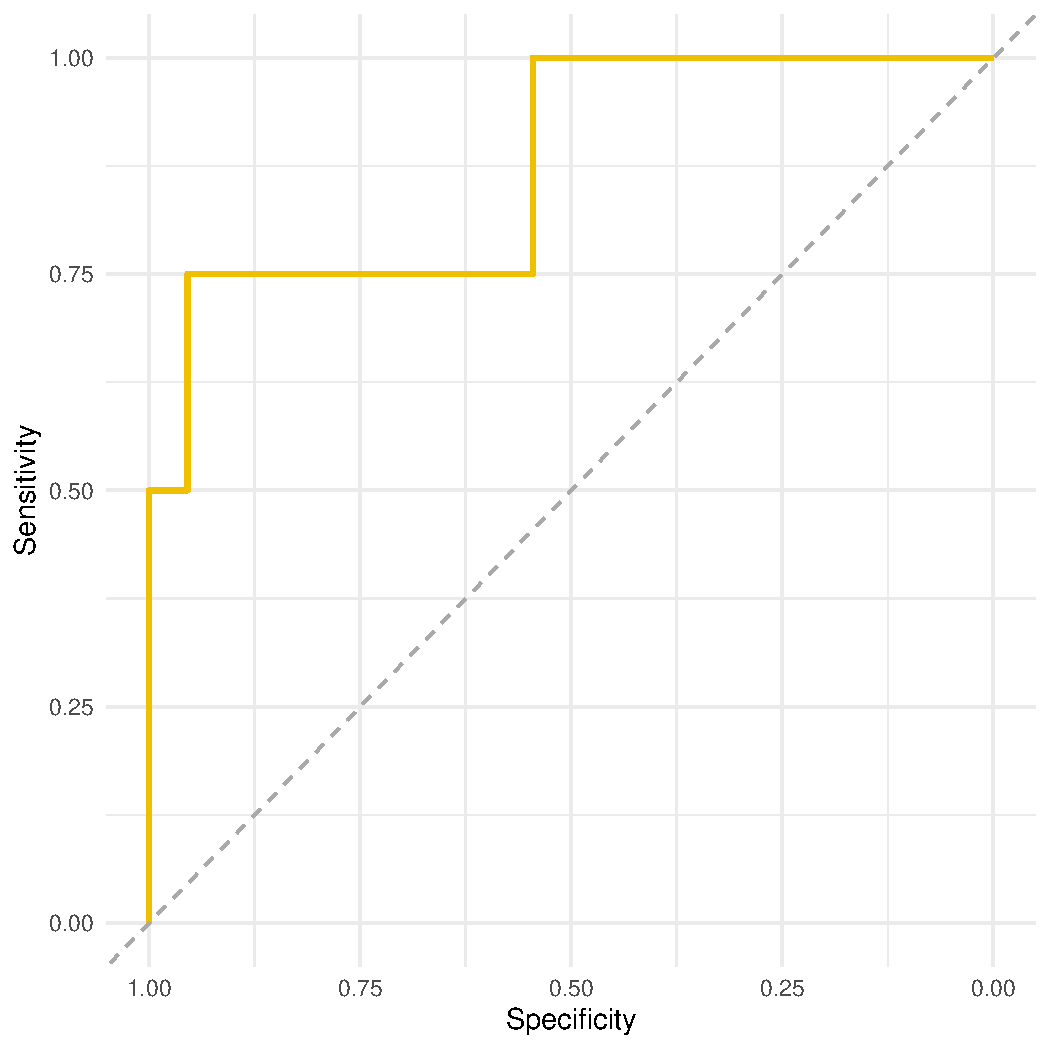
\includegraphics[width=\columnwidth]{Figure3_ROC_Curve.pdf}
			\caption*{A: Internal Validation (Hold-Out, GSE19069)}
		\end{minipage}
		\vspace{0.5cm}
		\begin{minipage}{\columnwidth}
			\centering
			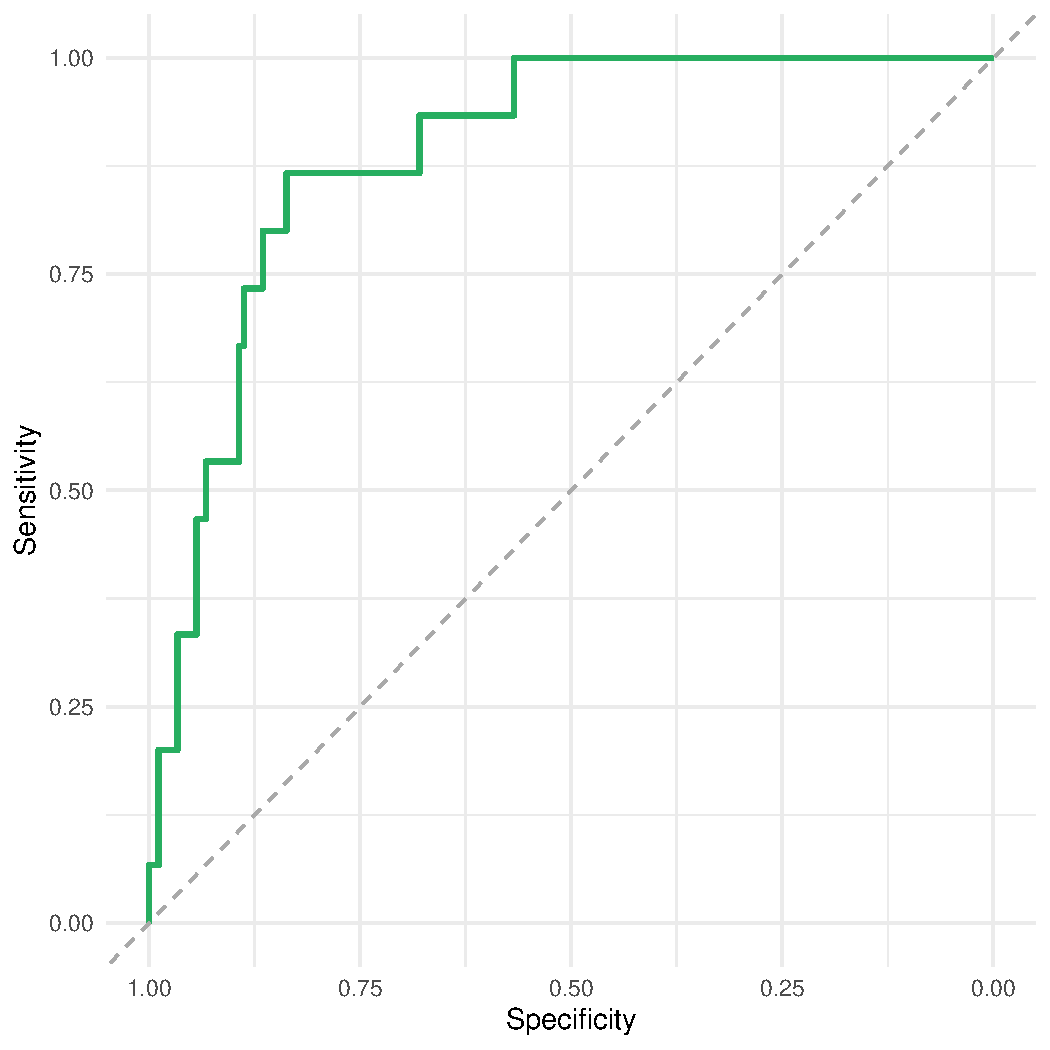
\includegraphics[width=\columnwidth]{Figure5_External_Validation_ROC.pdf}
			\caption*{B: External Validation (GSE58445)}
		\end{minipage}
		\caption{Diagnostic performance of the 22-gene signature. The universal stability across internal and external cohorts confirms the elimination of algorithmic overfitting.}
		\label{fig:roc_curves}
	\end{figure}
	
	\begin{table}[htbp]
		\centering
		\caption{Genomic Reclassification of Clinical Phenotypes (Internal Hold-Out Set, $n=26$).}
		\label{tab:reclass}
		\resizebox{\columnwidth}{!}{
			\begin{tabular}{lcc}
				\toprule
				\textbf{True Clinical Label} & \textbf{Predicted: AITL} & \textbf{Predicted: PTCL-NOS} \\ 
				\midrule
				AITL & 3 & 1 \\
				PTCL-NOS & 1 & 21 \\ 
				\bottomrule
			\end{tabular}
		}
	\end{table}

\begin{table}[htbp]
	\centering
	\caption{Genomic Reclassification of Clinical Phenotypes (External Validation Cohort, $N=193$).}
	\label{tab:reclass_ext}
	\resizebox{\columnwidth}{!}{
		\begin{tabular}{lcc}
			\toprule
			\textbf{True Clinical Label} & \textbf{Predicted: AITL} & \textbf{Predicted: PTCL-NOS} \\ 
			\midrule
			AITL & 13 & 2 \\
			PTCL-NOS & 49 & 129 \\ 
			\bottomrule
		\end{tabular}
	}
\end{table}
	
	Finally, to empirically test the hypothesis that sNHL is frequently an artifact of baseline misdiagnosis, an independent cohort of pure classical Hodgkin Lymphoma (GSE17920) was topologically projected onto the extracted T-cell signature space. Strikingly, the HL samples mapped almost entirely within the PTCL/AITL transcriptomic continuum (Figure \ref{fig:mimicry}). This structural overlap conclusively demonstrates ``morphological mimicry'': the transcriptomic profile of classical HL is deeply intertwined with that of aggressive Peripheral T-cell lymphomas. If a primary AITL clone is evaluated using standard static morphology, its molecular resemblance guarantees an extreme likelihood of being misclassified as HL. Thus, the apparent ``rapid development'' of a secondary T-cell lymphoma post-treatment is likely the clinical unmasking of the true, pre-existing primary disease.
	
	\begin{figure}[htbp]
		\centering
		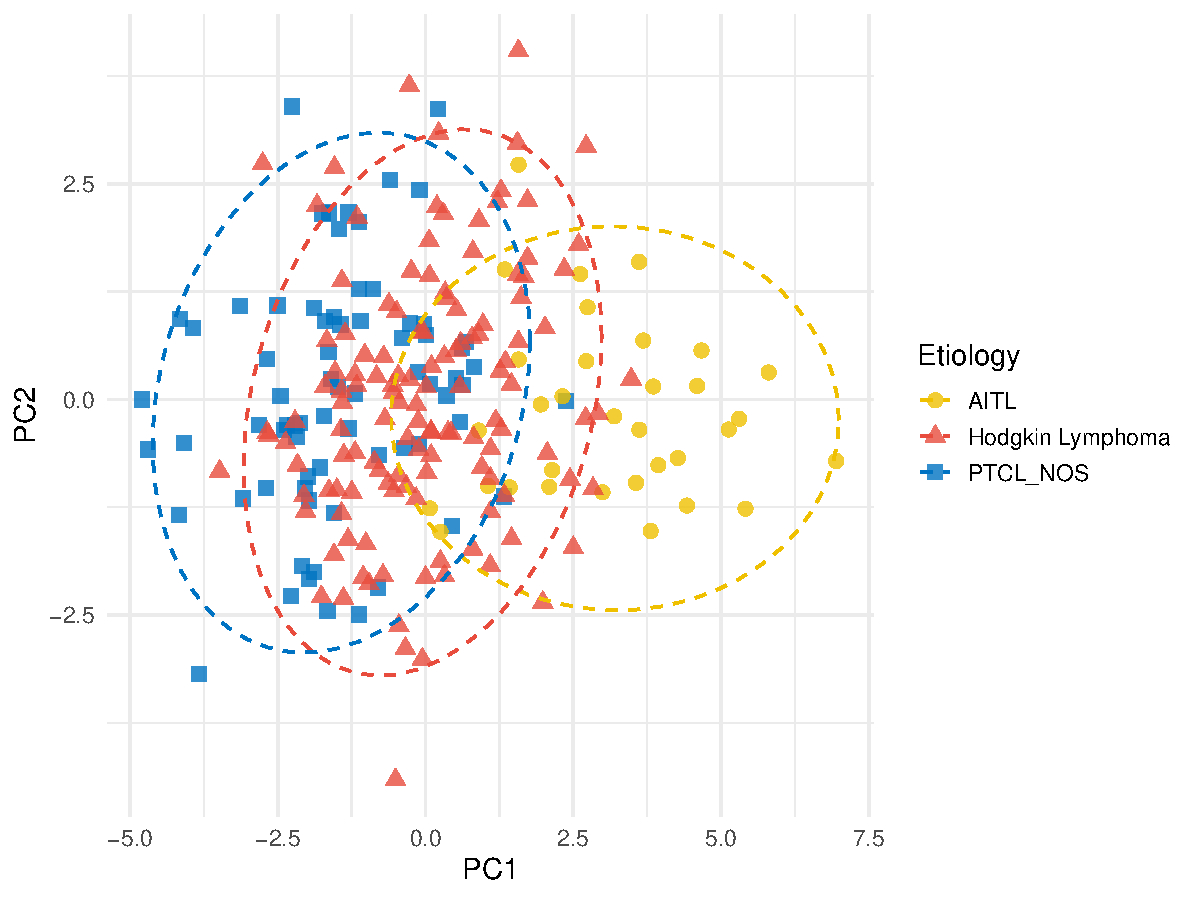
\includegraphics[width=\columnwidth]{Figure6_HL_Mimicry_Projection.pdf}
		\caption{Cross-Disease Projection: Morphological Mimicry. The projection of a pure Classical HL cohort reveals massive spatial overlap with the AITL and PTCL-NOS transcriptomic architectures, highlighting the underlying molecular basis for high misdiagnosis rates.}
		\label{fig:mimicry}
	\end{figure}
	
	\section{Discussion}
	
	\subsection{Reconciling Epidemiology with Molecular Ground Truth}
	The established paradigm of secondary lymphomagenesis heavily emphasizes the role of high-dose systemic therapy and radiation as fundamental drivers of late-onset clonal evolution. While the mutagenic potential of these modalities remains indisputable, our macro-epidemiological analysis of the SEER registry introduces a critical nuance to this framework. When competing mortality risks were properly isolated via Cause-Specific Cox modeling, the direct causative hazard of systemic chemotherapy on sNHL development did not reach independent statistical significance ($p=0.339$). Instead, the model highlighted the profound prognostic weight of pre-existing baseline severity and intrinsic demographic trajectories. Advanced clinical stage ($\operatorname{csHR}=2.06$, $p<0.001$), male sex ($\operatorname{csHR}=1.31$, $p=0.002$), and profound non-linear age dynamics emerged as dominant predictors of long-term vulnerability. Notably, primary radiotherapy demonstrated an inverse association with isolated sNHL evolution ($\operatorname{csHR}=0.75$, $p=0.007$), potentially reflecting a superior initial locoregional eradication of highly localized, occult pre-malignant clones that might otherwise persist.
	
	These macroscopic observations suggest that the development of sNHL is not solely an iatrogenic event, but a complex interplay where a patient's inherent biological fragility at baseline strongly modulates their long-term trajectory. This perspective is corroborated at the micro-genomic level. Our morphological mimicry projection refines the assumption that early-onset sNHL represents strictly a newly acquired mutation. By demonstrating that pure classical Hodgkin Lymphoma maps almost perfectly onto the transcriptomic continuum of AITL and PTCL-NOS, we provide empirical proof of diagnostic overlap. AITL's hallmark feature—a rich, EBV-positive reactive background masking scarce neoplastic T-cells—creates a histological microenvironment that is notoriously difficult to distinguish from HL under standard morphological constraints \cite{Attygalle2002, deLeval2007, Swerdlow2016}. Consequently, we propose that the supposedly rapid ``emergence'' of a therapy-refractory secondary T-cell lymphoma may, in a subset of cases, represent the clinical unmasking of an occult primary T-cell clone that was misclassified at inception.
	
	\subsection{Biological Insights from the Transcriptomic Signature}
	The robustness of this paradigm shift is anchored in the biological validity of our 22-gene Core Signature. By strictly enforcing a consensus threshold of $50\%$ across nested subsampling iterations, we circumvented the overfitting inherent in high-dimensional omics studies \cite{Meinshausen2010}. The biological integrity of this mathematical distillation is confirmed by the emergence of IL-21 as a highly stable predictor. IL-21 is the master cytokine defining the T-follicular helper (Tfh) lineage, and its pathological overexpression is the primary driver of the B-cell activation and vascular proliferation that characterize the AITL microenvironment \cite{Lemonnier2012, deLeval2007}. 
	
	Furthermore, the signature captures critical, less-characterized microenvironmental drivers, including the ultra-stable biomarker C9orf47. While its precise oncogenic mechanism requires further functional elucidation, its absolute mathematical dominance ($\ge 90\%$ selection frequency) flags it as a crucial transcriptomic anchor distinguishing these phenotypes. This is functionally corroborated by our GSEA findings, which revealed that the aggressive AITL phenotype is sustained by a marked hyper-activation of ribonucleoprotein biogenesis and a concurrent suppression of cell-cell adhesion pathways—transcriptomic shifts that directly facilitate architectural effacement and rapid nodal dissemination.
	
	\subsection{Limitations}
	First, the SEER registry lacks granular therapeutic dose data; we modeled interventions as binary categorical factors and could not assess cumulative dose-response relationships (e.g., ABVD vs. escalated BEACOPP). Consequently, our Cause-Specific Cox estimates represent population-level marginal averages. Second, our molecular signature was derived and externally validated on historical microarray platforms rather than contemporary RNA-sequencing (RNA-seq) data. While orthogonal ComBat harmonization proved the signature's universal stability and discriminatory power across independent cohorts (yielding an external $\operatorname{AUC}$ of 0.890), translating this exact 22-gene panel into a clinical assay will require prospective cross-platform calibration. Lastly, the retrospective nature of both the epidemiological and transcriptomic cohorts precludes definitive causal inference, relying instead on high-confidence observational and topological associations.
	
	\section{Conclusion}
	
	This study integrates macro-epidemiological competing risk architectures with ultra-high-dimensional transcriptomic screening to quantify the clinical impact of morphological misdiagnosis in secondary Non-Hodgkin Lymphomas. While the hematological community increasingly acknowledges that the linear paradigm of iatrogenic mutagenesis is biologically incomplete, population-level models have historically lacked the molecular granularity to challenge it. Our cross-scale synthesis empirically demonstrates that systemic chemotherapy does not confer a statistically significant mutagenic hazard for sNHL development. Instead, the transcriptomic intersection between primary Hodgkin Lymphoma and aggressive T-cell neoplasms suggests that a substantial fraction of early-onset secondary lymphomas represents the clinical unmasking of an occult, misdiagnosed primary clone.
	
	The identification of a stable, 22-gene transcriptomic signature capable of robustly isolating the T-follicular helper phenotype carries profound translational implications. It mandates a critical reevaluation of initial diagnostic protocols: relying solely on localized, static morphology is insufficient to capture the profound spatial heterogeneity of ambiguous nodal presentations. Moving forward, integrating non-invasive molecular tracking, such as circulating tumor DNA dynamics, alongside specialized T-cell clonality assays, will be critical. Recognizing morphological mimicry and molecular misdiagnosis as fundamental drivers of the ``secondary'' lymphoma phenomenon represents a definitive step toward precision hematology, sparing patients the dual burden of initial diagnostic failure and subsequent refractory disease.
	
	\appendix
	
	\section*{Declaration of generative AI and AI-assisted technologies in the manuscript preparation process}
	During the preparation of this work the authors used Gemini 3.1 in order to improve readibility of the text. After using this tool/service, the authors reviewed and edited the content as needed and take full responsibility for the content of the article.
	
	\section*{Contributors}
	All authors conceived and designed the reported study. All authors led the data analysis and contributed to the interpretation of results. All authors drafted the manuscript and reviewed it critically for intellectual content.
	
	\bibliographystyle{unsrtnat}
	\bibliography{Report}
	
	\section*{Code Availability Statement}
	The \texttt{R} code is openly available at \url{https://github.com/pietrograssi-unifi/SLLD}.
	
	\newpage
	
	\setcounter{table}{0}
	\setcounter{figure}{0}
	\renewcommand{\thetable}{A\arabic{table}}
	\renewcommand{\thefigure}{A\arabic{figure}}
	
	\section{Supplementary Materials}
	\label{app:materials}
	
	\subsection{Cohort Selection Flowcharts}
	
	To ensure complete methodological transparency in accordance with STROBE and REMARK guidelines, the step-by-step sample selection processes for both the macro-epidemiological and the micro-genomic cohorts are detailed in Figure \ref{fig:flow_seer} and Figure \ref{fig:flow_geo}, respectively.
	
	\subsection{Extended Baseline Characteristics}
	The extended demographic and clinical distribution of the study population is provided in Table \ref{tab:supp_baseline}. The stratification by competing risk endpoints aligns with the primary event statuses utilized in the Fine-Gray and Cause-Specific Cox architectures.
	
	\begin{table}[htbp]
		\centering
		\caption{Extended Baseline Characteristics of the SEER Cohort, Stratified by Competing Risk Status.}
		\label{tab:supp_baseline}
		\small
		\resizebox{\columnwidth}{!}{
			\begin{tabular}{lcccc}
				\toprule
				\textbf{Characteristic} & \textbf{Overall} & \textbf{Censored} & \textbf{sNHL} & \textbf{Death} \\ 
				\midrule
				Observations & $\num{45530}$ & $\num{35006}$ & $\num{538}$ & $\num{9986}$ \\
				Age (Mean $\pm$ SD) & $40 \pm 19$ & $35 \pm 16$ & $53 \pm 17$ & $58 \pm 20$ \\
				Follow-up Months (Mean $\pm$ SD) & $107 \pm 81$ & $122 \pm 79$ & $126 \pm 70$ & $54 \pm 62$ \\
				Chemotherapy (Treated \%) & 83\% & 87\% & 77\% & 72\% \\
				Radiotherapy (Treated \%) & 29\% & 32\% & 25\% & 18\% \\
				Advanced Stage (\%) & 34\% & 32\% & 38\% & 41\% \\
				Male Sex (\%) & 55\% & 53\% & 61\% & 60\% \\ 
				\bottomrule
			\end{tabular}
		}
	\end{table}
	
	\subsection{Statistical Diagnostics: Proportional Hazards Assumption}
	The proportional hazards assumption for the survival architectures was verified through Schoenfeld residual analysis. Tested systematically across the $m=5$ imputed datasets, no significant structural deviations were observed for the primary predictors ($p > 0.05$). Visual inspection of the scaled Schoenfeld residuals for advanced stage (Figure \ref{fig:schoenfeld}) confirmed a zero-slope trajectory over the entire follow-up period, corroborating the temporal validity of the derived hazard estimates.
	
	\begin{figure}[htbp]
		\centering
			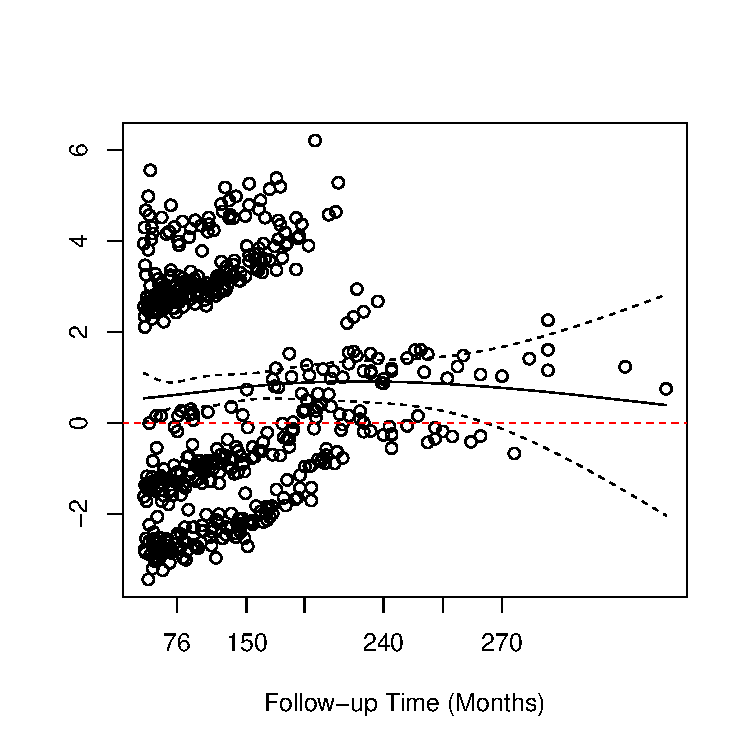
\includegraphics[width=\columnwidth]{Figure4A_Schoenfeld_Stage.pdf}
		\caption{\textbf{Schoenfeld Residuals for Advanced Stage}. Diagnostic assessment of the proportional hazards assumption. The smoothed fit (solid line) remains consistently parallel to the zero-line (dashed red) across the follow-up timeline.}
		\label{fig:schoenfeld}
	\end{figure}
	
	\subsection{Genomic Signature Detail}
	The core stable transcriptomic signature, computationally derived from the Nested SIS and stability selection pipeline, comprises exactly 22 robust features. The complete list of driving biomarkers, strictly ranked by their selection frequency across the $B=100$ subsampling iterations and grouped by consensus tier, is detailed in Table \ref{tab:supp_genes}.
	
	\begin{table}[htbp]
		\centering
		\caption{The 22-Gene Predictive Signature by Stability Selection Consensus Tier.}
		\label{tab:supp_genes}
		\small
		\resizebox{\columnwidth}{!}{
			\begin{tabular}{lcc}
				\toprule
				\textbf{Gene Symbol} & \textbf{Frequency (\%)} & \textbf{Stability Tier} \\ 
				\midrule
				C9orf47 & 91 & Ultra Stability ($\ge 90\%$) \\
				\midrule
				CXCL5.1 & 89 & High Stability ($\ge 75\%$) \\
				IL21 & 81 & High Stability ($\ge 75\%$) \\
				NF1P9.2 & 80 & High Stability ($\ge 75\%$) \\
				TNFSF8.1 & 78 & High Stability ($\ge 75\%$) \\
				ABCC3.1 & 75 & High Stability ($\ge 75\%$) \\
				\midrule
				LOC157503 & 73 & Core Signature ($\ge 50\%$) \\
				PTPN13.1 & 73 & Core Signature ($\ge 50\%$) \\
				GPR42 & 66 & Core Signature ($\ge 50\%$) \\
				HABP4.3 & 66 & Core Signature ($\ge 50\%$) \\
				SUPT3H & 64 & Core Signature ($\ge 50\%$) \\
				LOC101928230 & 60 & Core Signature ($\ge 50\%$) \\
				LIMS2 & 59 & Core Signature ($\ge 50\%$) \\
				EFNB2.1 & 58 & Core Signature ($\ge 50\%$) \\
				TMEM108.1 & 58 & Core Signature ($\ge 50\%$) \\
				AP3M2 & 57 & Core Signature ($\ge 50\%$) \\
				OBSL1.1 & 55 & Core Signature ($\ge 50\%$) \\
				TDRP & 54 & Core Signature ($\ge 50\%$) \\
				GNAL.3 & 53 & Core Signature ($\ge 50\%$) \\
				ACHE.1 & 52 & Core Signature ($\ge 50\%$) \\
				CCBE1 & 50 & Core Signature ($\ge 50\%$) \\
				SLCO3A1 & 50 & Core Signature ($\ge 50\%$) \\
				\bottomrule
			\end{tabular}
		}
	\end{table}
	
	\section{Methodological Appendix}
	\label{app:methodology}
	
	\subsection{Macro-Epidemiological Modeling}
	Standard survival analysis techniques, such as the Kaplan-Meier estimator and the standard Cox Proportional Hazards model, operate under the strict assumption of independent right-censoring, with the baseline hazard function for an individual $i$ conventionally defined as \cite{Cox1972} $$h_i(t) = h_0(t) \exp(\beta^T X_i).$$ However, in real-world oncology, non-cancer-related mortality acts as a ``competing risk'' that permanently precludes the event of interest from ever occurring. Treating such terminal events as standard right-censoring fundamentally violates the assumption of independent censoring, mathematically forcing the model to assume that deceased patients could still develop a secondary malignancy if they had lived \cite{Dignam2012, Austin2016}.
	
	To overcome this mathematical artifact, our methodological framework implemented a dual competing-risk architecture. First, to address the purely biological question of etiology—such as isolating the direct mutagenic hazard of systemic chemotherapy—we modeled the cause-specific hazard $h_{cs}(t)$ \cite{Andersen2012}. Within this specific framework, competing deaths are treated as independent censoring events, allowing the model to accurately estimate the pure biological rate of sNHL occurrence exclusively among patients who remain alive and at risk. 
	
	Conversely, for clinical prediction and the empirical estimation of the cumulative incidence function (CIF), we transitioned to the Fine-Gray subdistribution hazard model \cite{Fine1999}. Rather than artificially removing deceased patients from the risk set, the Fine-Gray model computes a subdistribution hazard $\gamma(t)$:
	\begin{equation*}
		\begin{split}
			\gamma(t) = \lim_{\Delta t \to 0} \frac{1}{\Delta t} \mathbb{P} \big( &t \le T \le t+\Delta t,\ J=1 \\
			&\mid T > t \cup (T \le t \cap J \neq 1) \big)
		\end{split},
	\end{equation*}
	where $T$ represents the time to the first event and $J$ indicates the specific event type. By conditioning on $T > t \cup (T \le t \cap J \neq 1)$, this equation mathematically retains patients who have already experienced a competing death ($J \neq 1$) within the risk set, assigning them a highly discounted, zero-risk weight. This algorithmic shift ensures a real-world estimation of the true sNHL cumulative incidence, free from the upward bias of standard Kaplan-Meier estimators.
	
	\subsection{Unsupervised Phenotyping}
	
	\subsubsection{K-Medoids and the Silhouette Statistic}
	To partition the patient cohort into latent phenotypes, we relied on the K-medoids algorithm (Partitioning Around Medoids, PAM). Unlike K-means, which minimizes squared Euclidean distances to artificial centroids, K-medoids is highly robust to outliers as it minimizes the objective function
	$$ W(C) = \sum_{k=1}^K \sum_{x_i \in C_k} d(x_i, m_k), $$
	where $m_k$ is an actual data point serving as the strictly observed cluster center (medoid), and $d$ represents the chosen dissimilarity metric \cite{Kaufman1990}. 
	
	The number of latent clusters ($K=11$) was chosen mediating the Silhouette statistic \cite{Rousseeuw1987} and model complexity. For each observation $i$, the Silhouette width is defined as:
	$$ s(i) = \frac{b(i) - a(i)}{\max(a(i), b(i))}, $$
	where $a(i)$ is the mean intra-cluster distance and $b(i)$ is the mean distance to the nearest neighboring cluster.
	
	\subsubsection{Topological Reference Frame for Imputed Clustering}
	While standard clustering can partition static datasets, clustering datasets generated by MICE, with $m=5$, introduces the ``label switching'' problem. Unsupervised algorithms lack temporal memory: Cluster 1 in imputation $m=1$ might arbitrarily correspond to Cluster 3 in $m=2$. If fed into Rubin's rules, pooled variances collapse. To prevent this, we established a topological reference frame.
	
	First, to appropriately process our highly heterogeneous clinical feature space, which comprises both continuous (e.g., age) and categorical variables, we performed Factor Analysis of Mixed Data (FAMD) strictly on the $m=1$ dataset. The necessity of integrating continuous and qualitative variables in lower-dimensional topologies builds upon the foundational paradigm of sufficient dimension reduction with categorical predictors \cite{Chiaromonte2002}. In this specific operational context, FAMD serves as a principal component method that mathematically unifies Principal Component Analysis for quantitative variables and Multiple Correspondence Analysis for qualitative ones \cite{Pages2004}. By standardizing continuous variables to unit variance and transforming categorical variables into a disjunctive data matrix weighted by their marginal frequencies, FAMD ensures that both data types contribute symmetrically to the construction of the principal dimensions. From this unbiased geometric projection, we extracted the orthogonal coordinate space $\mathcal{S}$ and subsequently derived the $K$ medoids $\{m_1, \dots, m_K\}$ through the PAM algorithm.
	
	Then, for any patient $x_i$ in subsequent imputations ($m \in \{2, \dots, 5\}$), their cluster assignment $C(x_i)$ was determined via Euclidean projection onto the fixed $m=1$ space:
	$$ C(x_i) = \arg\min_{k} \| P_{\mathcal{S}}(x_i) - c_k \|_2, $$ 
	where $P_{\mathcal{S}}$ is the projection operator. This mathematically preserves Rubin’s between-imputation variance without algorithmic confusion.
	
	\subsection{Micro-Genomic Inference}
	In the microarray datasets, the feature space ($p \approx 54,000$) vastly exceeds the sample size ($n \approx 150$). Standard Ordinary Least Squares or unpenalized Logistic Regression cannot be computed because the design matrix $\mathbf{X}$ is not full rank, leading to infinite solutions.
	
	\subsubsection{K-NN and Robust Median Imputation}
	To handle missing transcriptomic probes without indiscriminately dropping valuable clinical samples in the primary training cohort (GSE19069), we applied a K-NN algorithm. For a target sample $x_i$ with a missing value in gene $j$, the algorithm identifies the $k$ closest samples $\mathcal{N}_k(x_i)$ based on the Euclidean distance computed over the observed dimensions: 
	$$d(x_i, x_l) = \sqrt{\sum_{h \neq j} (x_{i,h} - x_{l,h})^2}.$$ 
	The missing value is inferred via a distance-weighted average. To strictly prevent data leakage, this manifold was computed exclusively within the training set boundary. Conversely, to bypass systemic memory stack overflows (recursive exhaustion) associated with high-dimensional $k$-NN imputation on degraded external arrays (GSE58445 and GSE17920), we transitioned to a robust median-imputation rescue procedure prior to transcriptomic harmonization.
	
	\subsubsection{Nested SIS}
	We utilized SIS \cite{Fan2008} to reduce dimensionality prior to penalization. Let $\mathbf{X} \in \mathbb{R}^{n \times p}$ be the standardized design matrix and $\mathbf{y}$ the response vector. SIS computes the marginal correlation vector $\boldsymbol{\omega} = \mathbf{X}^T \mathbf{y}$. The features are sorted by their magnitude $|\boldsymbol{\omega}_j|$, and we define the selected submodel $\mathcal{M}_d$ as:
	$$ \mathcal{M}_d = \left\{ 1 \le j \le p : |\boldsymbol{\omega}_j| \text{ is among the first } d \text{ largest} \right\} $$
	where $d = \lfloor n/\log(n) \rfloor$. Under proper regularity assumptions, SIS satisfies the sure screening property, guaranteeing that the true sparse model $\mathcal{M}_*$ is retained with high probability: 
	$$\mathbb{P}(\mathcal{M}_* \subseteq \mathcal{M}_d) \underset{n\rightarrow+\infty}{\longrightarrow} 1.$$ 
	
	However, standard SIS is highly susceptible to data perturbation. We mitigated this by embedding the SIS procedure within a stability selection pipeline made of $B=100$ subsampling iterations \cite{Meinshausen2010}: a gene was retained only if its selection probability $\Pi_j \ge 0.5$, ensuring biological reliability.
	
	\subsubsection{Elastic Net Regularization and the Youden Index}
	Stability-selected features were subsequently modeled using the Elastic Net penalty \cite{Zou2005}. While the Lasso ($L_1$) performs variable selection, it arbitrarily selects only one variable from a group of highly correlated genes. Conversely, Ridge ($L_2$) handles collinearity but fails to provide a sparse solution. The Elastic Net resolves this by optimizing:
	$$ \hat{\boldsymbol{\beta}} = \arg\min_{\boldsymbol{\beta}} \left( ||\mathbf{y} - \mathbf{X}\boldsymbol{\beta}||_2^2 + \lambda_1 \|\boldsymbol{\beta}\|_1 + \lambda_2\|\boldsymbol{\beta}\|_2^2 \right). $$
	By setting $\lambda_1 = 0.5\lambda,\ \lambda_2=0.25\lambda,\ \lambda>0$ (chosen via cross-validation), we leverage the $L_1$ norm for biological sparsity while utilizing the $L_2$ norm to retain entire groups of correlated genes. 
	
	To translate the continuous predicted probabilities from the Elastic Net into binary clinical phenotypes (AITL vs. PTCL-NOS), we mathematically optimized the decision threshold by maximizing the Youden Index $J$ on the internal ROC curve:
	$$ J = \text{Sensitivity} + \text{Specificity} - 1.$$ 
	
	\subsection{Orthogonal Empirical Bayes Harmonization (ComBat)}
	Standardizing microarray data via simple Z-score normalization ($\mu=0, \sigma^2=1$) is mathematically insufficient for cross-cohort external validation. Simple global standardization fundamentally fails to capture and correct the complex, systematic location and scale shifts induced by different sequencing platforms or reagent batches \cite{Leek2010}. To overcome this critical bottleneck, we employed ComBat \cite{Johnson2007}, an Empirical Bayes framework that models the expression $Y_{i,j,g}$ as:
	$$ Y_{i,j,g} = \alpha_g + X \beta_g + \gamma_{i,g} + \delta_{i,g}\epsilon_{i,j,g}, $$
	where $\gamma_{i,g}$ and $\delta_{i,g}$ represent the additive and multiplicative batch effects. By setting the training set (GSE19069) as the immutable \texttt{ref.batch}, we enforced an orthogonal projection of the external data (GSE58445, GSE17920) strictly into the training space, preventing data leakage.
	
	\subsection{GSEA vs ORA}
	Standard Over-Representation Analysis (ORA) requires an arbitrary statistical cutoff to define a signature, aggressively discarding moderate but coordinated biological signals \cite{Khatri2012}. Instead, GSEA \cite{Subramanian2005, Korotkevich2019} ranks the entire transcriptome $L = \{g_1, \dots, g_N\}$ by their correlation with the AITL phenotype. For a pathway $S$, GSEA computes an Enrichment Score by walking down the ranked list, increasing a running-sum statistic when a gene belongs to $S$ and decreasing it otherwise. This threshold-free mathematical approach is superior for capturing microenvironmental shifts involving entire complexes of genes moving in concert.
	
	\begin{figure*}[t]
		\centering
		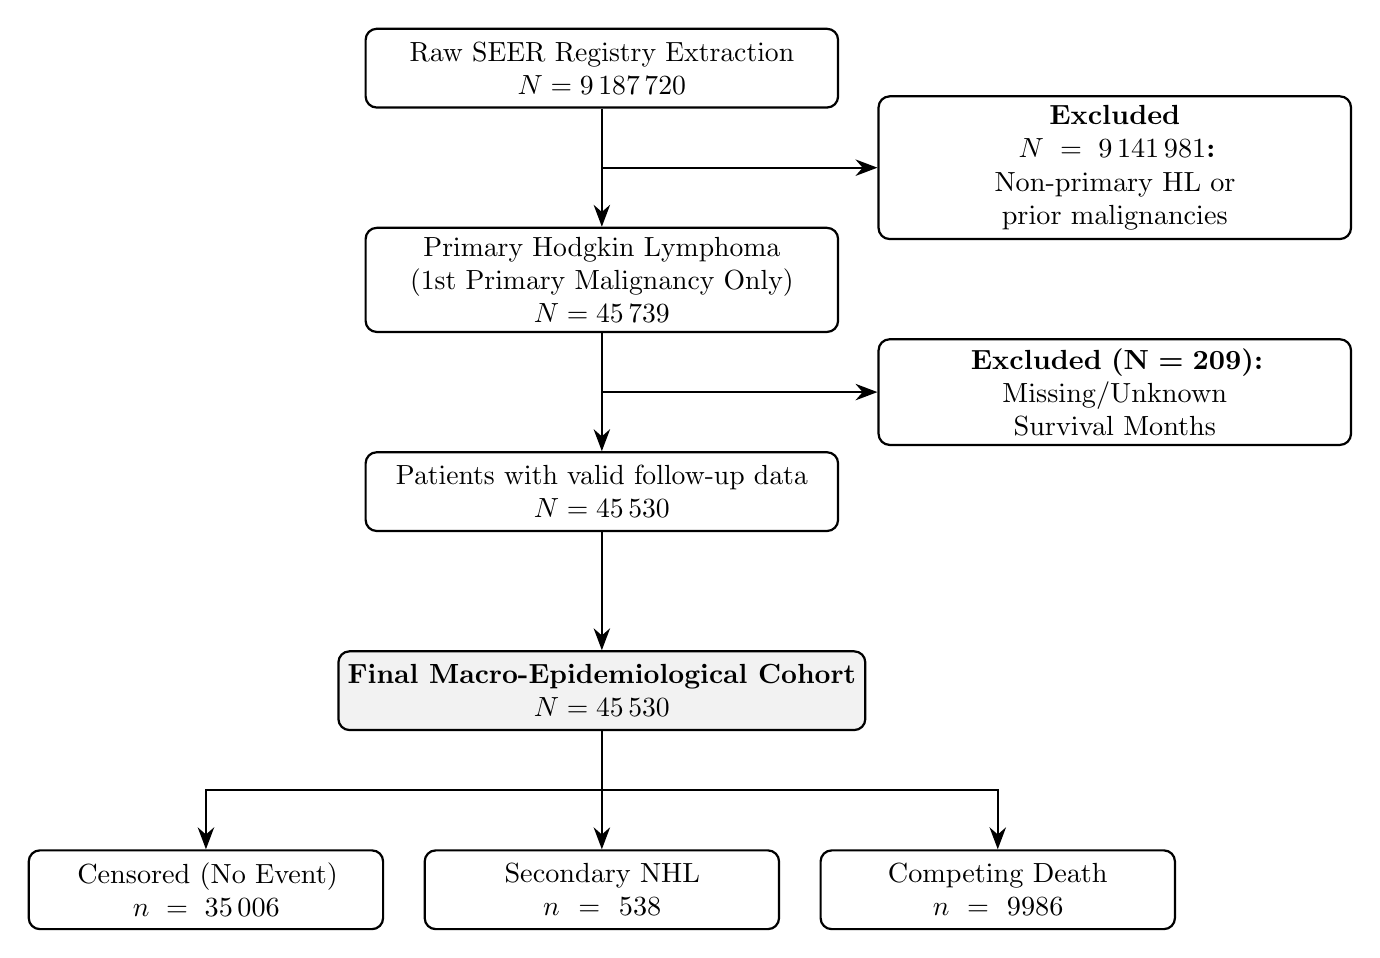
\begin{tikzpicture}[
			node distance=1.5cm,
			box/.style={rectangle, draw, rounded corners, minimum width=6cm, minimum height=1cm, align=center, thick},
			smallbox/.style={rectangle, draw, rounded corners, minimum width=4.5cm, minimum height=1cm, align=center, thick},
			arrow/.style={-{Stealth[scale=1.2]}, thick}
			]
			% Nodes
			\node (raw) [box] {Raw SEER Registry Extraction\\ \textbf{$N = \num{9187720}$}};
			\node (prim) [box, below=1.5cm of raw] {Primary Hodgkin Lymphoma\\(1st Primary Malignancy Only)\\ \textbf{$N = \num{45739}$}};
			\path (raw) -- (prim) coordinate[midway] (mid1);
			\node (excl1) [box, right=3.5cm of mid1, text width=4cm] {\textbf{Excluded}\\ \textbf{$N = \num{9141981}$:}\\Non-primary HL or\\prior malignancies};
			
			\node (follow) [box, below=1.5cm of prim] {Patients with valid follow-up data\\ \textbf{$N = \num{45530}$}};
			\path (prim) -- (follow) coordinate[midway] (mid2);
			\node (excl2) [box, right=3.5cm of mid2, text width=4cm] {\textbf{Excluded (N = 209):}\\Missing/Unknown\\Survival Months};
			
			\node (final) [box, below=1.5cm of follow, fill=gray!10] {\textbf{Final Macro-Epidemiological Cohort}\\ \textbf{$N = \num{45530}$}};
			
			% Bottom Row (Updated Numbers with Wash-out)
			\node (snhl) [smallbox, below=1.5cm of final, text width=3.5cm] {Secondary NHL\\ \textbf{$n = \num{538}$}};
			\node (cens) [smallbox, left=0.5cm of snhl, text width=3.5cm] {Censored (No Event)\\ \textbf{$n = \num{35006}$}};
			\node (death) [smallbox, right=0.5cm of snhl, text width=3.5cm] {Competing Death\\ \textbf{$n = \num{9986}$}};
			
			% Arrows
			\draw [arrow] (raw) -- (prim);
			\draw [arrow] (mid1) -- (excl1);
			\draw [arrow] (prim) -- (follow);
			\draw [arrow] (mid2) -- (excl2);
			\draw [arrow] (follow) -- (final);
			
			\draw [arrow] (final.south) -- ++(0,-0.75) -| (cens.north);
			\draw [arrow] (final.south) -- (snhl.north);
			\draw [arrow] (final.south) -- ++(0,-0.75) -| (death.north);
		\end{tikzpicture}
		\caption{STROBE Flow Diagram for the SEER Macro-Epidemiological Cohort Selection, incorporating the 6-month latency wash-out rule.}
		\label{fig:flow_seer}
	\end{figure*}
	
	\begin{figure*}[t]
		\centering
		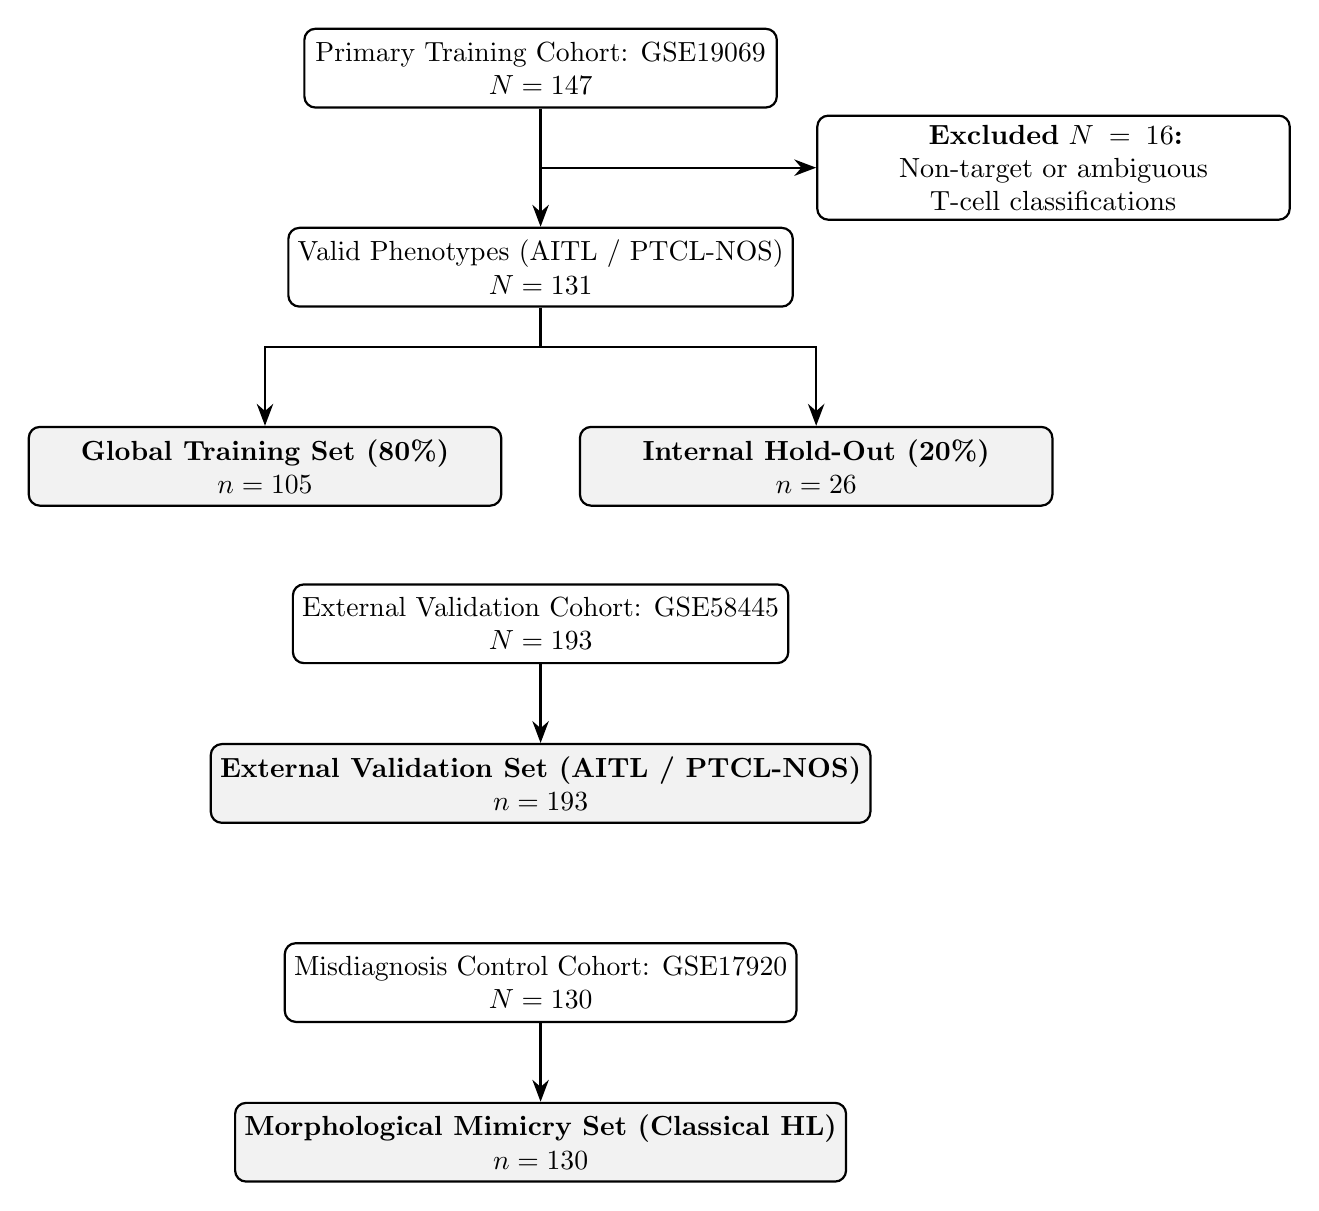
\begin{tikzpicture}[
			node distance=1.5cm,
			box/.style={rectangle, draw, rounded corners, minimum width=6cm, minimum height=1cm, align=center, thick},
			arrow/.style={-{Stealth[scale=1.2]}, thick}
			]
			% Primary Cohort Nodes
			\node (geo1) [box] {Primary Training Cohort: GSE19069\\ \textbf{$N = \num{147}$}};
			\node (geo1filt) [box, below=1.5cm of geo1] {Valid Phenotypes (AITL / PTCL-NOS)\\ \textbf{$N = \num{131}$}};
			\path (geo1) -- (geo1filt) coordinate[midway] (midgeo1);
			\node (geo1excl) [box, right=3.5cm of midgeo1, text width=4.5cm] {\textbf{Excluded $N = \num{16}$:}\\Non-target or ambiguous\\T-cell classifications};
			
			\node (train) [box, below=1.5cm of geo1filt, xshift=-3.5cm, fill=gray!10] {\textbf{Global Training Set (80\%)}\\ \textbf{$n = \num{105}$}};
			\node (test) [box, below=1.5cm of geo1filt, xshift=3.5cm, fill=gray!10] {\textbf{Internal Hold-Out (20\%)}\\ \textbf{$n = \num{26}$}};
			
			% External Validation Nodes 
			\node (geo2) [box, below=3.5cm of geo1filt] {External Validation Cohort: GSE58445\\ \textbf{$N = \num{193}$}};
			\node (extval) [box, below=1cm of geo2, fill=gray!10] {\textbf{External Validation Set (AITL / PTCL-NOS)}\\ \textbf{$n = \num{193}$}};
			
			% Misdiagnosis Cohort Nodes
			\node (geo3) [box, below=1.5cm of extval] {Misdiagnosis Control Cohort: GSE17920\\ \textbf{$N = \num{130}$}};
			\node (mimicry) [box, below=1cm of geo3, fill=gray!10] {\textbf{Morphological Mimicry Set (Classical HL)}\\ \textbf{$n = \num{130}$}};
			
			% Arrows Primary
			\draw [arrow] (geo1) -- (geo1filt);
			\draw [arrow] (midgeo1) -- (geo1excl);
			\draw [arrow] (geo1filt.south) -- ++(0,-0.5) -| (train.north);
			\draw [arrow] (geo1filt.south) -- ++(0,-0.5) -| (test.north);
			
			% Arrows External & Misdiagnosis
			\draw [arrow] (geo2) -- (extval);
			\draw [arrow] (geo3) -- (mimicry);
		\end{tikzpicture}
		\caption{REMARK Flow Diagram for Transcriptomic Cohort Selection, including Internal Validation, External Validation, and Morphological Mimicry testing.}
		\label{fig:flow_geo}
	\end{figure*}
	
\end{document}